\documentclass[11pt]{article}
\title{Meccano pentagons gallery}
\author{https://github.com/heptagons/meccano/penta/gallery}
\date{2023/12/18}

\usepackage{../../meccano}
\usepackage{amssymb}

\begin{document}

\maketitle
\begin{abstract}
We build rigid meccano\meccanoref regular pentagons from sides $3$ to $12$. We restrict all internal strips to remain inside the pentagon's perimeter and don't permit they overlap with others. We follow three steps. 1) We calculate distances between selected strips holes from the regular pentagon perimeter assuming is regular. 2) We run some programs available in this repo to look for rigid clusters of strips which contains the distance. 3) We simplify or reduce the cluster to fit inside the pentagon. We prove the correctness of the cluster distance applied to check the software. We try each construction is relevant for the pentagon size.
\end{abstract}

% 3

\section{Pentagons of size 3}

% 3-10
\subsection{Size 3 with 10 internal strips $build(3:3:1)$}

\begin{figure}[H]
\centering
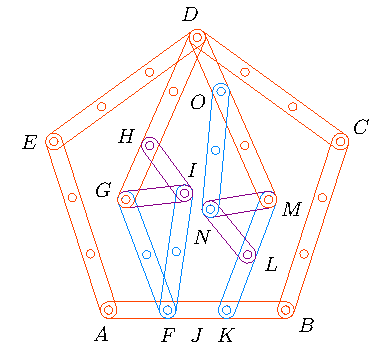
\includegraphics[scale=1.2]{3/penta3-10a}
\caption{Pentagon of size 3 with 10 internal strips. $\overline{DE}:\overline{EA}:\overline{AF} = 3:3:1$. $\overline{DF} = \overline{DK} = \dfrac{\sqrt{46+18\sqrt5}}2$.}
\label{fig:penta3-10a}
\end{figure}

Figure \ref{fig:penta3-10a} show the regular pentagon $A,B,C,D,E$ of size $3$. We know the regular pentagon height is side length times $\dfrac{\sqrt{5+2\sqrt5}}2$ so in this case $\overline{DJ} = \dfrac{3\sqrt{5+2\sqrt5}}2$ and we can calculate $\overline{DF}$:
\begin{align}
\overline{DF} &= \sqrt{(\overline{DJ})^2 + (\overline{FJ})^2}\nonumber\\
 &= \sqrt{\left(\frac{3\sqrt{5+2\sqrt5}}2\right)^2 + \left(\frac{1}2\right)^2}
 = \frac{\sqrt{46+18\sqrt5}}2
\end{align}

\subsubsection{Rigid distance $\dfrac{\sqrt{46+18\sqrt5}}2$}

Our five-strips software found several clusters and we use two different which fit inside the pentagon. We identify two angles $\alpha = \angle{HGI} = \angle{LMN}$ of equilateral triangles and $\beta = \angle{FGI} = \angle{NMO}$ of isoscelles'. Adding the angles we get angles $\angle{DGF} = \angle{DMK} = (\alpha + \beta)$. From equilateral triangle $\triangle{HGI}$ we calculate $\alpha$ and from isoscelles triangle $\triangle{FGI}$ we calculate $\beta$:
\begin{align}
\cos\alpha &= \frac{\overline{GI} / 2}{\overline{GH}} = \frac{1 / 2}1 = \frac{1}2\\
\sin\alpha &= \sqrt{1 - \cos^2\alpha} = \sqrt{1 - \left(\frac{1}2\right)^2} = \frac{\sqrt3}2\\
%
\cos\beta &= \frac{\overline{GI} / 2}{\overline{GF}} = \frac{1 / 2}2 = \frac{1}4\\
\sin\beta &= \sqrt{1 - \cos^2\beta} = \sqrt{1 - \left(\frac{1}4\right)^2} = \frac{\sqrt{15}}4
\end{align}

Finally we calculate $\cos(\alpha+\beta)$ with the sum identity and using the law of cosines we verify distance $\overline{DF}$:
\begin{align}
\cos(\alpha+\beta) &= \cos\alpha\cos\beta - \sin\alpha\sin\beta \nonumber\\
 &= \left(\frac{1}2\right)\left(\frac{1}4\right)
  -\left(\frac{\sqrt3}2\right)\left(\frac{\sqrt{15}}4\right)
 = \frac{1 - 3\sqrt5}8 \\
\overline{DF} &= \sqrt{(\overline{DG})^2 + (\overline{FG}^2)
 - 2(\overline{DG})(\overline{FG})\cos(\alpha+\beta)} \nonumber\\
 &= \sqrt{3^2 + 2^2 - 2(3)(2)\left(\frac{1 - 3\sqrt5}8\right)}
 = \frac{\sqrt{46+18\sqrt5}}2 \quad\blacksquare
\end{align}

% --- 3-14
\subsection{Size 3 with 14 internal strips $build(3:1)$}

\begin{figure}[H]
\centering
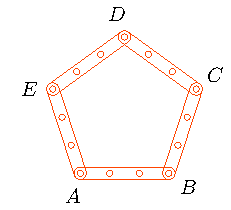
\includegraphics[scale=1.2]{3/penta3-14a}
\caption{Pentagon of size 3 with 14 internal strips. $\overline{AB}:\overline{BD} = 3:1$. $\overline{AD} = \dfrac{\sqrt{34+5\sqrt5}}2$.}
\label{fig:penta3-14a}
\end{figure}

Figure \ref{fig:penta3-14a} show the regular pentagon $A,B',A',C,B$ of size $3$. We know the internal angle of regular pentagon is $\theta \equiv \angle{ABD} = \dfrac{3\pi}5$ and $\cos\theta=\dfrac{1-\sqrt5}4$ so with the law of cosines we can calculate $\overline{AD}$ and the angle $\delta \equiv \angle{BAD}$:
\begin{align}
\overline{AD} &= \sqrt{(\overline{AB})^2 + (\overline{BD})^2
 - 2(\overline{AB})(\overline{BD})\cos\theta} \nonumber\\
 &= \sqrt{3^2 + 1^2 - 2(3)(1)\left(\frac{1-\sqrt5}4\right)} = \frac{\sqrt{34+6\sqrt5}}2\\
\cos\delta &= \frac{(\overline{AD})^2 + (\overline{AB})^2 - (\overline{BD})^2}
 {2(\overline{AD})(\overline{AB})} \nonumber\\
 &= \frac{\dfrac{34+6\sqrt5}4 + 3^2 - 1^2}{2\left(\dfrac{\sqrt{34+6\sqrt5}}2\right)(3)}
  = \frac{11+\sqrt5}{2\sqrt{34+6\sqrt5}}
\end{align}

\subsubsection{Rigid distance  $\dfrac{\sqrt{34+6\sqrt5}}2$}

Our five-strips software found several options to make the distance but we add manually a sixth strip in order to make a cluster narrow enough to fit two times inside the pentagon. The result is shown as cluster with vertices $DEFGH$ of figure \ref{fig:penta3-14a}. We prove the cluster's distance $\overline{AD}$ matches the distance alredy calculated.

We have a pair of adjacent equilateral triangles $\triangle{DGH}$ and $\triangle{EGH}$ so angle $\gamma \equiv \angle{DGE} = 2\pi / 3$ also $\cos\gamma = - 1/2$ so we can calculate $\overline{DE}$:
\begin{align}
\overline{DE} &= \sqrt{(\overline{DG})^2 + (\overline{GE})^2 
 - 2(\overline{DG})(\overline{GE})\cos\gamma} \nonumber\\
 &= \sqrt{1^2 + 1^2 - 2(1)(1)\left(-\frac{1}2\right)} = \sqrt3
\end{align}
We define angle $\alpha = \angle{GED}$ and calculate it using $\overline{DE}$:
\begin{align}
\cos\alpha &= \frac{(\overline{GE})^2 + (\overline{DE})^2 - (\overline{DG})^2}
 {2(\overline{GE})(\overline{DE})}
 = \frac{3 + 1^2 - 1^2}{2(\sqrt3)(1)} = \frac{\sqrt3}2\\
\sin\alpha &= \sqrt{1 - \cos^2\alpha} = \sqrt{1 - \left(\frac{\sqrt3}4\right)^2} 
 = \frac{1}2
\end{align}

From the isoscelles triangle $\triangle{AEF}$ we define angle $\epsilon \equiv \angle{AEF}$ noting $\cos\epsilon = \dfrac{\overline{EF}/2}{\overline{AE}} = \dfrac{1/2}{2} = \dfrac{1}4$ and we define angle $\beta \equiv \angle{AEG}$ the supplementary of $\epsilon$ and we get:
\begin{align}
\beta &= \pi - \epsilon \nonumber\\
\cos\beta &= -\cos\epsilon = -\frac{1}4 \\
\sin\beta &= \sqrt{1 - \cos^2\beta} = \sqrt{1 - \left(\frac{-1}4\right)^2} = \frac{\sqrt{15}}4
\end{align}

Finally we calculate the angle $\alpha + \beta$ with the sum identity plugin the last sines and cosines and use it to verify $\overline{AD}$ with the law of cosines:
\begin{align}
\cos(\alpha + \beta) &= \cos\alpha\cos\beta - \sin\alpha\sin\beta \nonumber\\
 & = \left(\frac{\sqrt3}2\right)\left(-\frac{1}4\right) 
  - \left(\frac{1}2\right)\left(\frac{\sqrt{15}}4\right) 
  = -\frac{\sqrt3 + \sqrt{15}}8 \\
\overline{AD} &= \sqrt{(\overline{DE})^2 + (\overline{EA})^2 
 - 2(\overline{DE})(\overline{EA})\cos(\alpha + \beta)} \nonumber\\
 &= \sqrt{3 + 2^2 - 2(\sqrt3)(2)\left(-\frac{\sqrt3 + \sqrt{15}}8\right)} 
 = \frac{\sqrt{34 + 6\sqrt5}}2 \quad\blacksquare
\end{align}

% 4

\section{Pentagons of size 4}

% 4-8
\subsection{Size 4 with 8 internal strips $build(2:4:1:2)$}

\begin{figure}[H]
\centering
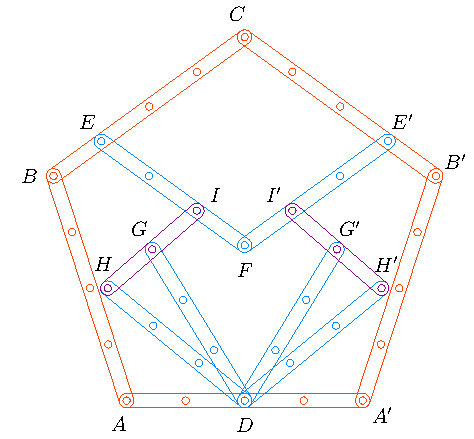
\includegraphics[scale=1.1]{4/penta4-8a}
\caption{Pentagon of size 4 with 6 internal strips. $\overline{DA} : \overline{AB} : \overline{BE} : \overline{EI} = 2:4:1:2$. $\overline{DI} = \sqrt{11}$.}
\label{fig:penta4-8a}
\end{figure}

Figure \ref{fig:penta4-8a} show the regular pentagon $AA'B'CB$ of size $4$. We calculate the distance $\overline{DI}$ assuming vertex $D$ is at origin and calculating abscissa and ordinate of vertex $I$ and knowing $\alpha = \angle{ADB} = 3\pi / 5$ and $\beta = \angle{B'BE} = \pi / 5$. Adding and substracting through vertices $DABEI$ we get:
\begin{align}
I_x &= -\overline{DA} - \overline{AB}|\cos\alpha| + \overline{BE}\cos\beta + \overline{EI}\cos\beta \nonumber\\
 &= -2 -(4)\left(\frac{\sqrt5 - 1}4\right) + (1+2)\left(\frac{\sqrt5+1}4\right)
 = -\frac{1+\sqrt5}4 \\
I_y &= \overline{AB}\sin\alpha + \overline{BE}\sin\beta - \overline{BI}\sin\beta \nonumber\\
 &= (4)\left(\frac{\sqrt{10+2\sqrt5}}4\right) + (1-2)\left(\frac{\sqrt{10-2\sqrt5}}4\right)
 = \frac{4\sqrt{10+2\sqrt5} - \sqrt{10-2\sqrt5}}4 \\
%
\overline{DI} &= \sqrt{(I_x - D_x)^2 + (I_y - I_y)^2} \nonumber\\
 &= \frac{\sqrt{(1+\sqrt5)^2 + (4\sqrt{10+2\sqrt5} - \sqrt{10-2\sqrt5})^2}}4
 = \sqrt{11}
\end{align}

\subsubsection{Rigid distance $\sqrt{11}$}

Our three-strips software found several clusters for distance $\sqrt{11}$. We prove the selected cluster $DHGI$ inside the pentagon of figure \ref{fig:penta4-8a} matches the expected distance. First we calculate the angle $\alpha \equiv \angle{DHG}$ with the law of cosines and use the value to finally verify the distance $\overline{DI}$ with again the law of cosines:
\begin{align}
\cos\alpha &= \frac{(\overline{HD})^2 + (\overline{HG})^2 - (\overline{DG})^2}
 {2(\overline{HD})(\overline{HG})} \nonumber\\
 &= \frac{3^2 + 1^2 - 3^2}{2(3)(1)} = \frac{1}6 \\
\overline{DI} &= \sqrt{(\overline{HD})^2 + (\overline{HI})^2
 - 2(\overline{HD})(\overline{HD})\cos\alpha} \nonumber\\
 &= \sqrt{3^2 + 2^2 - 2(3)(2)\left(\frac{1}6\right)} = \sqrt{11} \quad\blacksquare
\end{align}

% 4-10
\subsection{Size 4 with 10 internal strips $build(3:4)$}

\begin{figure}[H]
\centering
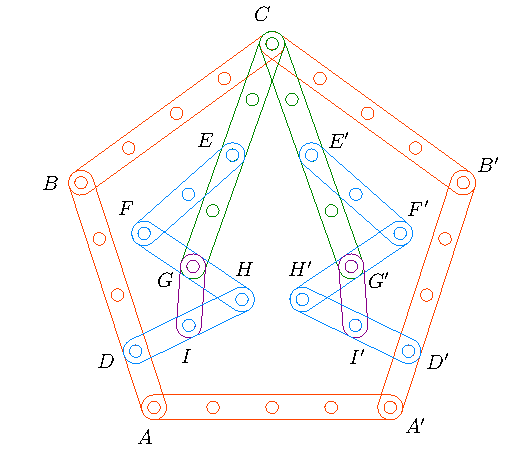
\includegraphics[scale=1.1]{4/penta4-10a}
\caption{Pentagon of size 4 with 10 internal strips. $\overline{CB} : \overline{BD} = 4:3$. $\overline{CD} = \sqrt{19 + 6\sqrt5}$.}
\label{fig:penta4-10a}
\end{figure}

Figure \ref{fig:penta4-10a} show the regular pentagon $A,A',B',C,B$ of size $4$. We know the internal angle of pentagon is $\theta=\angle{CBD}=\dfrac{3\pi}5$ and $\cos\theta=\dfrac{1-\sqrt5}4$ so with the law of cosines we can calculate $\overline{CD}$ and the angle $\delta = \angle{BDC}$:
\begin{align}
\overline{CD} &= \sqrt{(\overline{BC})^2 + (\overline{BD})^2
 - 2(\overline{BC})(\overline{BD})\cos\theta} \nonumber\\
 &= \sqrt{4^2 + 3^2 - 2(4)(3)\left(\frac{1-\sqrt5}4\right)} = \sqrt{19+6\sqrt5}\\
%
\cos\delta &= \frac{(\overline{CD})^2 + (\overline{BC})^2 - (\overline{BD})^2}
 {2(\overline{CD})(\overline{BC})} \nonumber\\
 &= \frac{(19+6\sqrt5) + 4^2 - 3^2}{2\left(\sqrt{19+6\sqrt5}\right)(4)}
  = \frac{13 + 3\sqrt5}{4\sqrt{19+6\sqrt5}}
\end{align}

\subsubsection{Rigid distance  $\sqrt{19+6\sqrt5}$}

Our five-strips software found several clusters for distance $\sqrt{19+6\sqrt5}$. We prove selected cluster $CEFGHID$ show in the figure \ref{fig:penta4-10a} matches pentagon's distace $\overline{CD}$. Set the cluster in the coordinate plane such that vertice $G$ is at the origin and vertices $F$ at $(-1,0)$ and vertice $H$ at $(+1,0)$.
Since triangle $\triangle{EFG}$ is isoscelles and $\overline{CG}$ is the double of $\overline{GE}$ we know angle $\angle{CFG} = \pi / 2$ and we can calculate the abscissa and ordinate of vertex $C$:
\begin{align}
C_x &= -\overline{FG} = -1 \\
C_y &= \sqrt{(\overline{CG})^2 - (\overline{FG})^2} = \sqrt{4^2 - 1^2} = \sqrt{15}
\end{align}

Since triangle $\triangle{GHI}$ is equilateral and $\overline{HD}$ is the double of $\overline{HI}$ we know angle $\angle{DGH} = \pi / 2$ and we can calculate the abscissa and ordinate of vertex $D$:
\begin{align}
D_x &= 0 \\
D_y &= -\sqrt{(\overline{HD})^2 - (\overline{GH})^2} = -\sqrt{2^2 - 1^2} = -\sqrt3
\end{align}

Finally we verify the distance $\overline{CD}$
\begin{align}
\overline{CD} &= \sqrt{(C_x - D_x)^2 + (C_y - D_y)^2} \nonumber\\
 &= \sqrt{(-1 - 0)^2 + (\sqrt{15} + \sqrt{3})^2} = \sqrt{19 + 6\sqrt5} \quad\blacksquare
\end{align}

% 5

\section{Pentagons of size 5}

% 5-10
\subsection{Size 5 with 10 internal strips $build(3,5)$}

\begin{figure}[H]
\centering
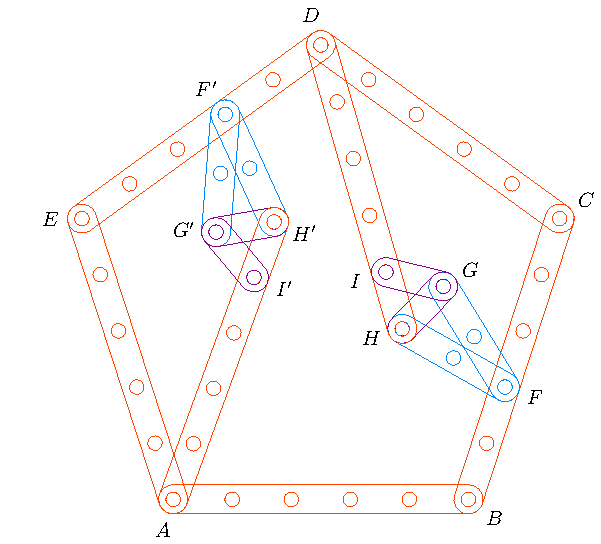
\includegraphics[scale=0.9]{5/penta5-10a}
\caption{Pentagon of size 5 with 10 internal strips. $\overline{FC} : \overline{CD} = 3:5$. $\overline{FD} = \dfrac{\sqrt{106 + 30\sqrt5}}2$.}
\label{fig:penta5-10a}
\end{figure}

Figure \ref{fig:penta5-10a} show the regular pentagon $ABCDE$ of size $5$. We know the internal angle of pentagon $\theta=\angle{FCD} =\dfrac{3\pi}5$ and $\cos\theta=\dfrac{1-\sqrt5}4$ so with the law of cosines we can calculate $\overline{FD}$ and the angle $\delta = \angle{CFD}$:
\begin{align}
\overline{FD} &= \sqrt{(\overline{FC})^2 + (\overline{CD})^2
 - 2(\overline{FC})(\overline{CD})\cos\theta} \nonumber\\
 &= \sqrt{3^2 + 5^2 - 2(3)(5)\left(\frac{1-\sqrt5}4\right)} = \frac{\sqrt{106 + 30\sqrt5}}2\\
%
\cos\delta &= \frac{(\overline{FD})^2 + (\overline{FC})^2 - (\overline{CD})^2}
 {2(\overline{FD})(\overline{FC})} \nonumber\\
 &= \frac{\left(\dfrac{106+30\sqrt5}4\right) + 3^2 - 5^2}
  {2\left(\dfrac{\sqrt{106+30\sqrt5}}2\right)(3)}
  = \frac{7 + 5\sqrt5}{2\sqrt{106 + 30\sqrt5}}
\end{align}


\subsubsection{Rigid distance $\dfrac{\sqrt{106 + 30\sqrt5}}2$}

Our five-strips software found the cluster $FGHID$ of figure \ref{fig:penta5-10a}. We calculate two angles, angle $\alpha \equiv \angle{FHG}$ within isoscelles triangle $\triangle{FHG}$ and angle $\beta \equiv \angle{GHI}$ within equilateral triangle $\triangle{GHI}$:
\begin{align}
\cos\alpha &= \frac{\overline{HG}/2}{\overline{FH}} = \frac{1/2}2 = \frac{1}4 \\
\sin\alpha &= \sqrt{1 - \cos^2\alpha} = \sqrt{1 - \left(\frac{1}4\right)^2} = \frac{\sqrt{15}}4\\
%
\cos\beta &= \frac{\overline{HG}/2}{\overline{HI}} = \frac{1/2}{1} = \frac{1}2 \\
\sin\beta &= \sqrt{1 - \cos^2\beta} = \sqrt{1 - \left(\frac{1}2\right)^2} = \frac{\sqrt{3}}2
\end{align}

Finally we calculte angle $\angle{FHD} = \alpha + \beta$ with the cosines sum identity and use it to verify the distance $\overline{FD}$ using the law of cosines:
\begin{align}
\cos(\alpha+\beta) &= \cos\alpha\cos\beta - \sin\alpha\sin\beta \nonumber\\
 &= \left(\frac{1}4\right)\left(\frac{1}2\right) 
  - \left(\frac{\sqrt{15}}4\right)\left(\frac{\sqrt{3}}2\right)
  = \frac{1 - 3\sqrt{5}}8 \\
\overline{FD} &= \sqrt{(\overline{FH})^2 + (\overline{HD})^2 
 - 2(\overline{FH})(\overline{HD})\cos(\alpha + \beta)} \nonumber\\
 &= \sqrt{2^2 + 5^2 - 2(2)(5)\left(\frac{1 - 3\sqrt{5}}8\right)}
 = \frac{\sqrt{106 + 30\sqrt5}}2 \quad \blacksquare
\end{align}


% 5-12
\subsection{Size 5 with 12 internal strips $build(4:5:4)$}

\begin{figure}[H]
\centering
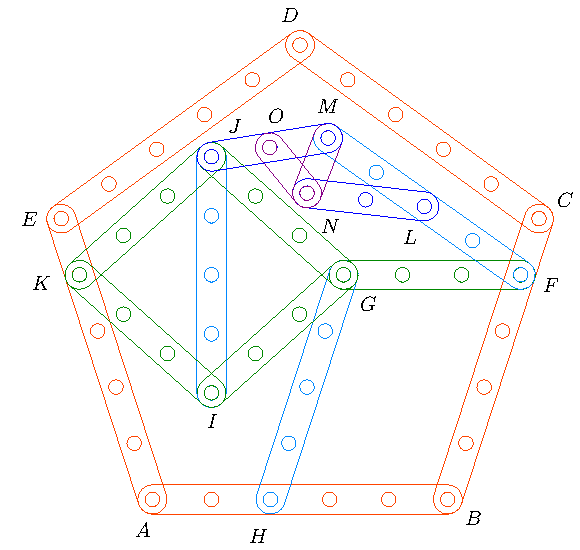
\includegraphics[scale=0.9]{5/penta5-12a}
\caption{Pentagon of size 5 with 12 internal strips. $\overline{FB} : \overline{BA} : \overline{AK} = 4:5:4$ and $\overline{FK} = 3 + 2\sqrt5$. $\overline{FJ} = \sqrt{18+6\sqrt5} = \sqrt3 + \sqrt{15}$.}
\label{fig:penta5-12a}
\end{figure}

Figure \ref{fig:penta5-12a} show pentagon $ABCDE$ of size $5$. For this construction we need vertices $K,G,F$ to be collinear. First we note the three consecutive sides: $\overline{KA}$, $\overline{AS}$ and $\overline{SR}$ of an (incomplete) sub-pentagon and we know its \textbf{width} $\overline{KR}$ equals $\dfrac{1+\sqrt5}2$ times the side $\overline{KA}$ so here $\overline{KR} = 2 + 2\sqrt5$ and we have:
\begin{align}
\overline{KF} &= \overline{KR} + \overline{RF} = 3 + 2\sqrt5
\end{align}

Strip $\overline{GH}$ is parallel and of the same size of $\overline{FB}$ so makes rigid vertices $A$ and $B$ once colliner vertices $K,G,F$ are rigid which we will show next.

\subsubsection{Rigid distance $3+2\sqrt5$}

In figure \ref{fig:penta5-12a} we have an isoscelles triangle $\triangle{GIJ}$ and we calculate $\overline{PG} = \sqrt{(\overline{GI})^2 - (\overline{PI})^2} = \sqrt{3^2 - 2^2} = \sqrt5$. Similarly the other isoscelles triange $\triangle{IJK}$ gives $\overline{PK} = \sqrt{5}$ so we have (iff $K,P,G,F$ were collinear):
\begin{align}
\overline{KF} = \overline{KP} + \overline{PG} + \overline{GF} = 3 + 2\sqrt5 \quad \blacksquare
\end{align}

Vertices $K,P,G$ already are collinear. For $P,G,F$ collinearity we need two angles $\alpha \equiv \angle{PGJ}$ and $\beta \equiv \overline{FGJ}$ with the condition $\alpha + \beta = \pi$. Within isoscelles triangle $\triangle{GIJ}$ we calculate $\alpha$ and then $\beta$ (its supplement) and use $\beta$ to calculate the distance $\overline{FJ}$ with the law of cosines:
\begin{align}
\cos\alpha &= \frac{\overline{PG}}{\overline{GJ}} = \frac{\sqrt5}3 \\
\cos\beta &= -\cos\alpha = -\frac{\sqrt5}3 \\
\overline{FJ} &= \sqrt{(\overline{FG})^2 + (\overline{GJ})^2
 - 2(\overline{FG})(\overline{GJ})\cos\beta} \nonumber\\
 &= \sqrt{3^2 + 3^2 - 2(3)(3)\left(-\frac{\sqrt5}3\right)}
 = \sqrt{18 + 6\sqrt5}
\end{align}

With extra five-strips cluster $FLMNOJ$ distance $FJ$ is made rigid as we show in next section.

\subsubsection{Rigid distance $\sqrt{18+6\sqrt5} = \sqrt3 + \sqrt{15}$}

Our five-strips software generated among other solutions the cluster $FLMNOJ$ of figure \ref{fig:penta5-12a}. This cluster makes rigid the other cluster $FGJIK$. Here we validate the five-strips cluster. We have the equilateral triangle $\triangle{MNO}$ and $\overline{MJ}$ is the double of $\overline{MO}$ so angle $\angle{MNJ} = \pi/2$. Similarly we have the isoscelles triangle $\triangle{MNL}$ and $\overline{MF}$ is the double of $\overline{ML}$ so angle $\angle{MNF} = \pi/2$. With the two right angles vertices $J,N,F$ are collinear so we can calculate easily $\overline{FJ}$:
\begin{align}
\overline{FJ} &= \overline{JN} + \overline{NF} \nonumber\\
 &= \sqrt{(\overline{JM})^2 - (\overline{MN})^2} 
  + \sqrt{(\overline{FM})^2 - (\overline{MN})^2} \nonumber\\
 &= \sqrt{2^2 - 1^2} + \sqrt{4^2 - 1^2} = \sqrt{3} + \sqrt{15} 
 = \sqrt{18 + 6\sqrt5} \quad \blacksquare
\end{align}

% 6

\section{Pentagons of size 6}

% 6-6
\subsection{Size 6 with 6 internal strips $build(4:6:4)$}

\begin{figure}[H]
\centering
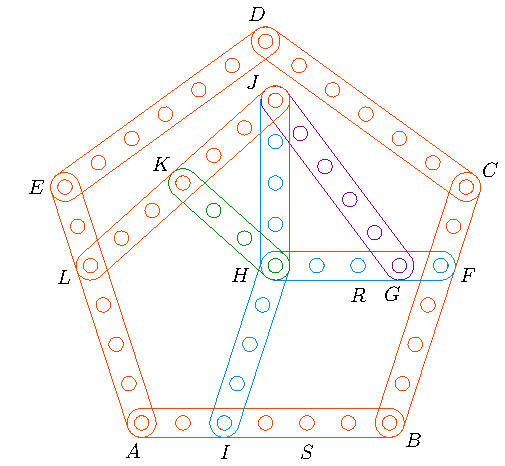
\includegraphics[scale=1]{6/penta6-6a}
\caption{Pentagon of size 6 with 6 internal strips. $\overline{FB} : \overline{BA} : \overline{AL} = 4:6:4$. $\overline{FL} = 4 + 2\sqrt5$.}
\label{fig:penta6-6a}
\end{figure}

Figure \ref{fig:penta6-6a} show pentagon $ABCDE$ of size $5$. For this construction we need vertices $L,H,F$ to be collinear. First we note the three consecutive sides: $\overline{LA}$, $\overline{AS}$ and $\overline{SR}$ of a (incomplete) sub-pentagon and we know its \textbf{width} $\overline{LR}$ equals $\dfrac{1+\sqrt5}2$ times the side $\overline{LA}$ so here $\overline{LR} = 2 + 2\sqrt5$ and we can have:
\begin{align}
\overline{LF} = \overline{LR} + \overline{RF} = 4 + 2\sqrt5
\end{align}

Strip $\overline{HI}$ is parallel and of the same size of $\overline{FB}$ so makes rigid vertices $A$ and $B$.

\subsubsection{Rigid distance $4 + 2\sqrt5$}

In figure \ref{fig:penta6-6a} we have two right angles. First angle $\angle{LHJ} = \pi / 2$ because triangle $\triangle{HJK}$ is isoscelles and $\overline{JL}$ is the double of $\overline{JK}$. Second angle $\angle{FHJ} = \pi / 2$ because $\triangle{GHJ}$ is Pythagorean. Then vertices $L,H,F$ are colliear and we can calculate $\overline{LH}$:
\begin{align}
\overline{LF} &= \overline{LH} + \overline{HF} \nonumber\\
 &= \sqrt{(\overline{LJ})^2 - (\overline{JH})^2} + 4 
 = \sqrt{6^2 - 4^2} + 4 = 4 + 2\sqrt5 \quad \blacksquare
\end{align}

% 6-8a
\subsection{Size 6 with 8 internal strips $build(6:6:3:4)$}

\begin{figure}[H]
\centering
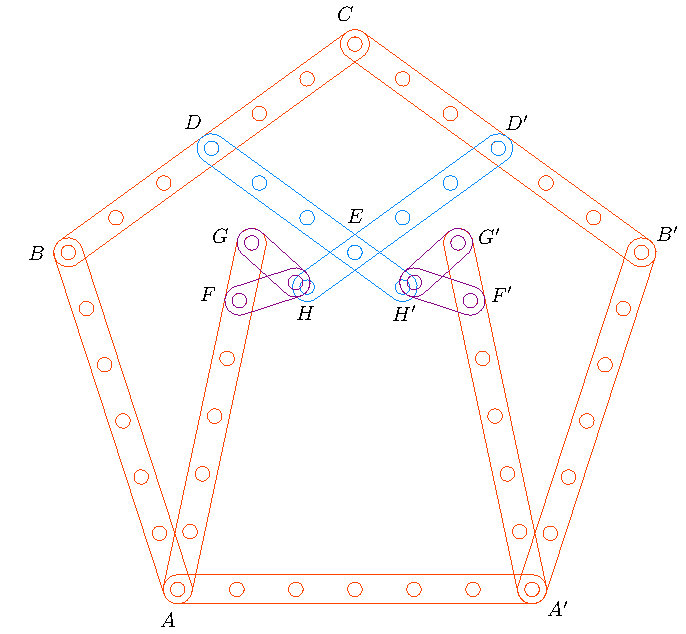
\includegraphics[scale=1]{6/penta6-8a}
\caption{Pentagon of size 6 with 8 internal strips. $\overline{A'A} : \overline{AB} : \overline{BD} : \overline{DH'} = 6:6:3:4$ and $\overline{A'H'} = \sqrt{31}$.}
\label{fig:penta6-8a}
\end{figure}

Figure \ref{fig:penta6-8a} show the regular pentagon $AA'B'CB$ of size $6$. We calculate the distance $\overline{A'H'}$ assuming vertex $A'$ is at origin and calculating abscissa and ordinate of vertex $H'$. We define $\alpha \equiv \angle{ADB} = 3\pi / 5$ and $\beta \equiv \angle{B'BE} = \pi / 5$ and add and substract through vertices $A',A,B,D,H'$ to get:
\begin{align}
H'_x &= -\overline{A'A} -\overline{AB}|\cos\alpha| + \overline{BD}\cos\beta + \overline{DH}\cos\beta \nonumber\\
 &= -6 -(6)\left(\frac{\sqrt5 - 1}4\right) + (3+4)\left(\frac{\sqrt5+1}4\right)
 = \frac{-11 + \sqrt5}4 \\
H'_y &= \overline{AB}\sin\alpha + \overline{BD}\sin\beta - \overline{DH'}\sin\beta \nonumber\\
 &= (6)\left(\frac{\sqrt{10+2\sqrt5}}4\right) + (3-4)\left(\frac{\sqrt{10-2\sqrt5}}4\right)
 = \frac{6\sqrt{10+2\sqrt5} - \sqrt{10-2\sqrt5}}4 \\
%
\overline{A'H'} &= \sqrt{(H'_x)^2 + (H'_y)^2} \nonumber\\
 &= \frac{\sqrt{(-11+\sqrt5)^2 + (6\sqrt{10+2\sqrt5} -\sqrt{10-2\sqrt5})^2}}4
 = \sqrt{31}
\end{align}

\subsubsection{Rigid distance $\sqrt{31}$}

Our three-strips software found the cluster $AFGH$ in the figure which fits inside this pentagon. We define angle $\theta \equiv \angle{FGH} = \pi / 3$ since triangle $\triangle{FGH}$ is equilateral so $\cos\theta = 1 / 2$ and we can verify $\overline{AH}$ with the law of cosines:
\begin{align}
\overline{AH} &= \sqrt{(\overline{GH})^2 + (\overline{AG})^2 
 - 2(\overline{GH})(\overline{AG})\cos\theta} \nonumber\\
 &= \sqrt{1^2 + 6^2 - 2(1)(6)\left(\frac{1}2\right)} = \sqrt{31} \quad \blacksquare
\end{align}

% 6-8b
\subsection{Size 6 with 8 internal strips $build(3:6:4:6)$}

\begin{figure}[H]
\centering
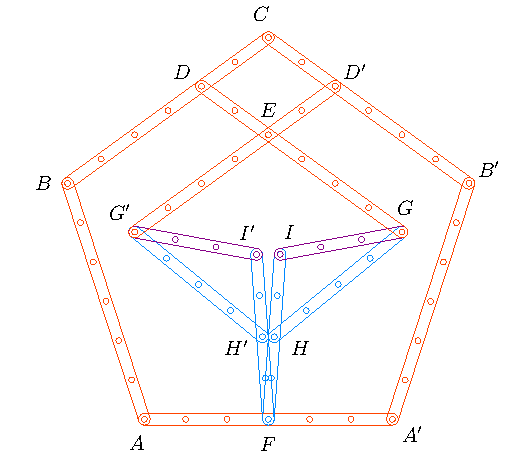
\includegraphics[scale=1.2]{6/penta6-8b}
\caption{Pentagon of size 6 with 8 internal strips. $\overline{FA} : \overline{AB} : \overline{BD} : \overline{DG} = 3:6:4:6$ and $\overline{FG} = \sqrt{31}$.}
\label{fig:penta6-8b}
\end{figure}

Figure \ref{fig:penta6-8b} show the regular pentagon $AA'B'CB$ of size $6$. We calculate the distance $\overline{FG}$ assuming vertex $F$ is at origin and calculating abscissa and ordinate of vertex $G$. We define $\alpha \equiv \angle{A'AB} = 3\pi / 5$ and $\beta \equiv \angle{B'BD} = \pi / 5$ and add and substract ortogonal distances through vertices $F,A,B,D,G$ to get:
\begin{align}
G_x &= -\overline{FA} -\overline{AB}|\cos\alpha| + \overline{BD}\cos\beta + \overline{DG}\cos\beta \nonumber\\
 &= -3 -(6)\left(\frac{\sqrt5 - 1}4\right) + (4+6)\left(\frac{\sqrt5+1}4\right)
 = \frac{4 + 4\sqrt5}4 \\
G_y &= \overline{AB}\sin\alpha + \overline{BD}\sin\beta - \overline{DG}\sin\beta \nonumber\\
 &= (6)\left(\frac{\sqrt{10+2\sqrt5}}4\right) + (4-6)\left(\frac{\sqrt{10-2\sqrt5}}4\right)
 = \frac{6\sqrt{10+2\sqrt5} - 2\sqrt{10-2\sqrt5}}4 \\
%
\overline{FG} &= \sqrt{(G_x)^2 + (G_y)^2} \nonumber\\
 &= \frac{\sqrt{(4+4\sqrt5)^2 + (6\sqrt{10+2\sqrt5} -2\sqrt{10-2\sqrt5})^2}}4
 = \sqrt{31}
\end{align}

\subsubsection{Rigid distance $\sqrt{31}$}

Our three-strips software found the cluster $FGHI$ that fits (hardly) inside the pentagon in the figure. With the law of cosines we calculate angle $\theta = \angle{IHG}$ and then we use the supplement (cosine negative) as $\angle{FHG}$ to verify $\overline{FG}$, again with the law of cosines:
\begin{align}
\cos\theta &= \frac{(\overline{HG})^2 + (\overline{HI})^2 - (\overline{IG})^2}
 {2(\overline{HG})(\overline{HI})} \nonumber\\
 &= \frac{4^2 + 2^2 - 3^2}{2(4)(2)} = \frac{11}{16} \\
\overline{FG} &= \sqrt{(\overline{FH})^2 + (\overline{HG})^2 
 - 2(\overline{FH})(\overline{HG})(-\cos\theta) } \nonumber\\
 &= \sqrt{2^2 + 4^2 - 2(2)(4)\left(-\frac{11}{16}\right)}
 = \sqrt{31} \quad \blacksquare
\end{align}

% 6:10
\subsection{Size 6 with 10 internal strips $build(5:6)$}

\begin{figure}[H]
\centering
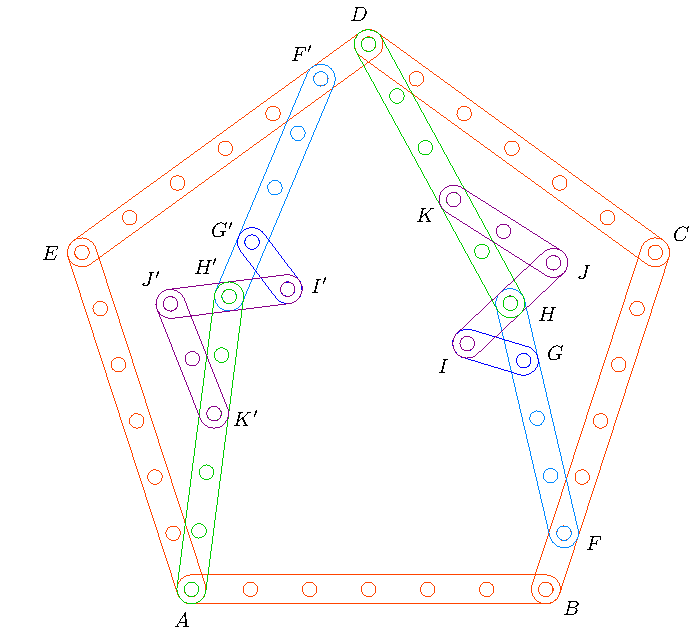
\includegraphics[scale=1]{6/penta6-10a}
\caption{Pentagon of size 6 with 10 internal strips. $\overline{FC} : \overline{CD} = 5:6$. $\overline{FD} = \sqrt{46 + 15\sqrt5}$.}
\label{fig:penta6-10a}
\end{figure}

Figure \ref{fig:penta6-10a} show the regular pentagon $ABCDE$ of size $6$. We know the internal angle of pentagon $\theta=\angle{FCD} =\dfrac{3\pi}5$ and $\cos\theta=\dfrac{1-\sqrt5}4$ so with the law of cosines we can calculate $\overline{FD}$ and the angle $\delta = \angle{CFD}$:
\begin{align}
\overline{FD} &= \sqrt{(\overline{FC})^2 + (\overline{CD})^2
 - 2(\overline{FC})(\overline{CD})\cos\theta} \nonumber\\
 &= \sqrt{5^2 + 6^2 - 2(5)(6)\left(\frac{1-\sqrt5}4\right)} = \sqrt{46 + 15\sqrt5}\\
%
\cos\delta &= \frac{(\overline{FD})^2 + (\overline{FC})^2 - (\overline{CD})^2}
 {2(\overline{FD})(\overline{FC})} \nonumber\\
 &= \frac{\left(46 + 15\sqrt5\right) + 5^2 - 6^2}
  {2\left(\sqrt{46 + 15\sqrt5}\right)(5)}
  = \frac{7 + 3\sqrt5}{2\sqrt{46 + 15\sqrt5}}
\end{align}

\subsubsection{Rigid distance $\sqrt{46 + 15\sqrt5}$}

Our five-strips software found cluster $FGHIJKD$ shown in figure \ref{fig:penta6-10a}. Suppose vertice $H$ is at the origin while vertice $I$ is at $\{-1,0\}$ and vertice $J$ is at $\{+1,0\}$. Triangle $\triangle{HJK}$ is isoscelles so we can found the coordinates of vertice $K$ and vertice $D$ which is a scaled coordinate of $K$ by a factor $\overline{DH} / \overline{KH}$:
\begin{align}
K\{x,y\} &= \left\{\frac{\overline{HJ}}2, 
 \sqrt{(\overline{HK})^2 - \left(\frac{\overline{HJ}}2\right)^2}\right\} \nonumber\\
 &= \left\{\frac{1}2, \sqrt{2^2 - \left(\frac{1}2\right)^2}\right\} 
 = \left\{\frac{1}2,\frac{\sqrt{15}}2\right\} \\
%
D\{x,y\} &= \left(\frac{\overline{DH}}{\overline{KH}}\right)K\{x,y\} \nonumber\\
 &= \left(\frac{5}2\right)\left\{\frac{1}2,\frac{\sqrt{15}}2\right\}
 = \left\{ \frac{5}4 , \frac{5\sqrt{15}}4 \right\}
\end{align}

Triangle $\triangle{GHI}$ is equilateral so we can found the coordinates of vertice $G$ and vertice $F$ which is a scaled coordinate of $G$ by factor of $\overline{HF} / \overline{GF}$:
\begin{align}
G\{x,y\} &= \left\{ -\frac{\overline{HI}}2, 
 - \sqrt{(\overline{HG})^2 - \left( \frac{\overline{HI}}2 \right)^2}\right\} \nonumber\\
 &= \left\{ -\frac{1}2, -\sqrt{1^2 - \left(\frac{1}2\right)^2} \right\}
 = \left\{ -\frac{1}2, -\frac{\sqrt3}2 \right\} \\
%
F\{x,y\} &= \left(\frac{\overline{HF}}{\overline{GF}}\right)G\{x,y\} \nonumber\\
 &= \left(4\right)\left\{ -\frac{1}2, -\frac{\sqrt3}2 \right\}
 = \left\{ -2, -2\sqrt{3} \right\}
\end{align}

Finally we verify the distance $\overline{FD}$:
\begin{align}
\overline{FD} &= \sqrt{(D_x - F_x)^2 + (D_y - F_y)^2} \nonumber\\
 &= \sqrt{ \left( \frac{5}4 -(-2) \right)^2 
  + \left( \frac{5\sqrt{15}}4 -(-2\sqrt{3}) \right)^2}
 = \sqrt{46 + 15\sqrt{5}} \quad \blacksquare
\end{align}

% --- 6:12
\subsection{Size 6 with 12 internal strips $build(0:6:4:2)$}

\begin{figure}[H]
\centering
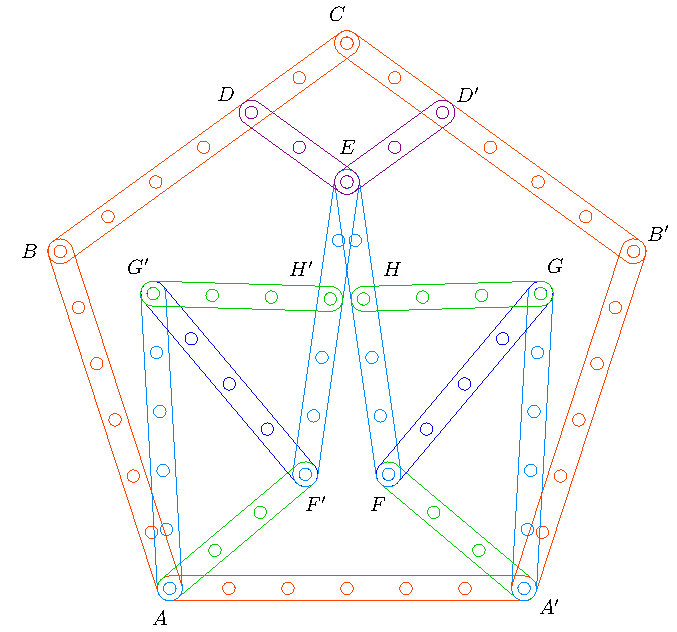
\includegraphics[scale=1]{6/penta6-12a}
\caption{Pentagon of size 6 with 12 internal strips. $\overline{AA}:\overline{AB}:\overline{BD}:\overline{DE} = 0:6:4:2$ and $AE = \sqrt{34 + 10\sqrt5}$} 
\label{fig:penta6-12a}
\end{figure}

Figure \ref{fig:penta6-12a} show the regular pentagon $AA'B'CB$ of size $6$. We calculate the distance $\overline{AE}$ assuming vertex $A$ is at origin and calculating abscissa and ordinate of vertex $E$. We define $\alpha \equiv \angle{A'AB} = 3\pi / 5$ and $\beta \equiv \angle{B'BC} = \pi / 5$ and add and substract orthogonal distances through vertices $ABDE$ to get:
\begin{align}
E_x &= -\overline{AB}|\cos\alpha| + \overline{BD}\cos\beta + \overline{DE}\cos\beta \nonumber\\
 &= -(6)\left(\frac{\sqrt5 - 1}4\right) + (4+2)\left(\frac{\sqrt5+1}4\right)
 = \frac{12}4 \\
E_y &= \overline{AB}\sin\alpha + \overline{BD}\sin\beta - \overline{DE}\sin\beta \nonumber\\
 &= (6)\left(\frac{\sqrt{10+2\sqrt5}}4\right) + (4-2)\left(\frac{\sqrt{10-2\sqrt5}}4\right)
 = \frac{6\sqrt{10+2\sqrt5} + 2\sqrt{10-2\sqrt5}}4 \\
%
\overline{AE} &= \sqrt{(E_x)^2 + (E_y)^2} \nonumber\\
 &= \frac{\sqrt{(12)^2 + (6\sqrt{10+2\sqrt5} +2\sqrt{10-2\sqrt5})^2}}4
 = \sqrt{34 + 10\sqrt5}
\end{align}

\subsubsection{Rigid distance $\sqrt{34 + 10\sqrt5}$}

Our five-strips sofware found the cluster $AFGHE$ shown in figure \ref{fig:penta6-12a}. We define two angles $\alpha \equiv \angle{AFG} = \pi/2$ within the Pythagorean triangle $\triangle{AFG}$ and $\beta \equiv \angle{GFH}$ within isoscelles triangle $\triangle{GFH}$ so we have:
\begin{align}
\cos\alpha &= 0\\
\sin\alpha &= 1\\
\cos\beta &= \frac{\overline{GF} / 2}{\overline{FH}} = \frac{4/2}{3} = \frac{2}3\\
\sin\beta &= \sqrt{1 - \cos^2\beta} = \sqrt{1 - \left(\frac{2}3\right)^2} = \frac{\sqrt5}3
\end{align}

Finally we calculate $\angle{AFE} = \alpha + \beta$ with the cosine sum identity and use it to verify the distance $\overline{AE}$ with the law of cosines:
\begin{align}
\cos(\alpha+\beta) &= \cos\alpha\cos\beta - \sin\alpha\sin\beta \nonumber\\
 &= (0)\left(\frac{2}3\right) - (1)\left(\frac{\sqrt5}3\right) = -\frac{\sqrt5}3 \\
%
\overline{AE} &= \sqrt{(\overline{AF})^2 + (\overline{FE})^2 
 - 2(\overline{AF})(\overline{FE})\cos(\alpha + \beta)} \nonumber\\
 &= \sqrt{3^2 + 5^2 - 2(3)(5)\left(-\frac{\sqrt5}3\right)}
 = \sqrt{34 + 10\sqrt5} \quad \blacksquare
\end{align}

% === 7 ===

\section{Pentagons of size 7}

% 7-6
\subsection{Size 7 with 6 internal strips $build(6:7:6)$}

\begin{figure}[H]
\centering
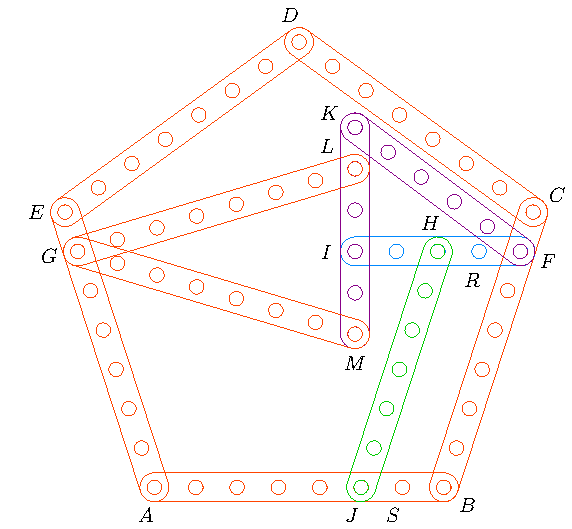
\includegraphics[scale=1]{7/penta7-6a}
\caption{Pentagon of size 7 with 6 internal strips. $\overline{FC} : \overline{CD} : \overline{} = 6:7:6$. $\overline{FD} = 4 + 3\sqrt5$.}
\label{fig:penta7-6a}
\end{figure}

Figure \ref{fig:penta7-6a} show pentagon $ABCDE$ of size $7$. For this construction we need vertices $G,I,F$ to be collinear. First we note the three consecutive sides: $\overline{GA}$, $\overline{AS}$ and $\overline{SR}$ of an (incomplete) sub-pentagon of size $6$. We know its \textbf{width} $\overline{GR}$ equals $\dfrac{1+\sqrt5}2$ times the side $\overline{GA}$ so here $\overline{GR} = 3 + 3\sqrt5$ and then:
\begin{align}
\overline{GF} &= \overline{GR} + \overline{RF} = 4 + 3\sqrt5
\end{align}

Strip $\overline{HJ}$ is parallel and of the same size of $\overline{FB}$ so makes rigid vertices $A$ and $B$ once vertices $G,I,F$ were rigid.

\subsubsection{Rigid distance $4 + 3\sqrt5$}

In figure \ref{fig:penta7-6a} triangle $\triangle{GLM}$ is isoscelles so angle $\angle{GIL} = \pi / 2$ and triangle $\triangle{FIK}$ is Pythagorean so angle $\angle{FIK} = \pi / 2$. With the two right angles the vertices $G,I,F$ are collinear and we can easily verify distance $\overline{GF}$:
\begin{align}
\overline{GF} &= \overline{GI} + \overline{IF} \nonumber\\
 &= \sqrt{(\overline{GL})^2 - (\overline{LI})^2} + 4 
 = \sqrt{7^2 - 2^2} + 4 = 4 + 3\sqrt{5} \quad \blacksquare
\end{align}

% 7-10
\subsection{Size 7 with 10 internal strips $build(6,7)$}

\begin{figure}[H]
\centering
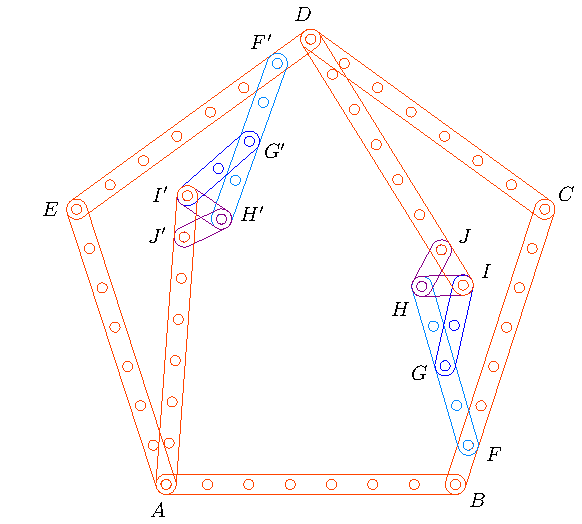
\includegraphics[scale=1]{7/penta7-10a}
\caption{Pentagon of size 7 with 10 internal strips. $\overline{FC}:\overline{CD} = 6:7$. $\overline{FD} = \sqrt{64 + 21\sqrt5}$.}
\label{fig:penta7-10a}
\end{figure}


Figure \ref{fig:penta7-10a} show the regular pentagon $ABCDE$ of size $7$. We know the internal angle of pentagon $\theta=\angle{FCD} =\dfrac{3\pi}5$ and $\cos\theta=\dfrac{1-\sqrt5}4$ so with the law of cosines we can calculate $\overline{FD}$ and the angle $\delta = \angle{CFD}$:
\begin{align}
\overline{FD} &= \sqrt{(\overline{FC})^2 + (\overline{CD})^2
 - 2(\overline{FC})(\overline{CD})\cos\theta} \nonumber\\
 &= \sqrt{6^2 + 7^2 - 2(6)(7)\left(\frac{1-\sqrt5}4\right)} = \sqrt{64 + 21\sqrt5}\\
%
\cos\delta &= \frac{(\overline{FD})^2 + (\overline{FC})^2 - (\overline{CD})^2}
 {2(\overline{FD})(\overline{FC})} \nonumber\\
 &= \frac{\left(64 + 21\sqrt5\right) + 6^2 - 7^2}
  {2\left(\sqrt{64 + 21\sqrt5}\right)(6)}
  = \frac{17 + 7\sqrt5}{4\sqrt{64 + 21\sqrt5}}
\end{align}

\subsubsection{Rigid distance $\sqrt{64 + 21\sqrt5}$}

Our five-strips software produced the cluster $FGHIJD$ shown in figure \ref{fig:penta7-10a}. Consider vertice $I$ at origin $(0,0)$ and vertice $H$ at coordinate $(-1,0)$. Since triangle $\triangle{GHI}$ is isoscelles and $\overline{HF}$ is the double of ${FG}$ we have angle $\angle{HIF} = \pi/2$ and we can calculate the coordinates of vertice $F$ as:
\begin{align}
F_x &= 0 \\
F_y &= \overline{IF} \nonumber\\
 &= -\sqrt{(\overline{HF})^2 - (\overline{HI})^2} = -\sqrt{4^2 - 1^2} = -\sqrt{15}
\end{align}

Since triangle $\triangle{HIJ}$ is equilateral we have this coordinates for vertice $J$:
\begin{align}
J_x = -\overline{IJ}\cos(\pi/3) = -(1)\frac{1}2 = -\frac{1}2 \\
J_y = +\overline{IJ}\sin(\pi/3) = (1)\frac{\sqrt3}2 = \frac{\sqrt3}2
\end{align}
We notice vertice $D$ is a coordinate scaled from vertice $J$ by a factor of $\overline{DI} / \overline{JI} = 7$ so $D_x = -7/2$ and $D_y = 7\sqrt3 / 2$. Finally we verify the distance $\overline{FD}$ using the coordinates values of vertices $F,D$:
\begin{align}
\overline{FD} &= \sqrt{(D_x - F_x)^2 + (D_y - F_y)^2} \nonumber\\
 &= \sqrt{\left(-\frac{7}2 - 0\right)^2 + \left( \frac{7\sqrt3}2 - (-\sqrt{15})\right)^2}
 = \sqrt{64 + 21\sqrt5} \quad \blacksquare
\end{align}

% 7-14
\subsection{Size 7 with 14 internal strips}

\begin{figure}[H]
\centering
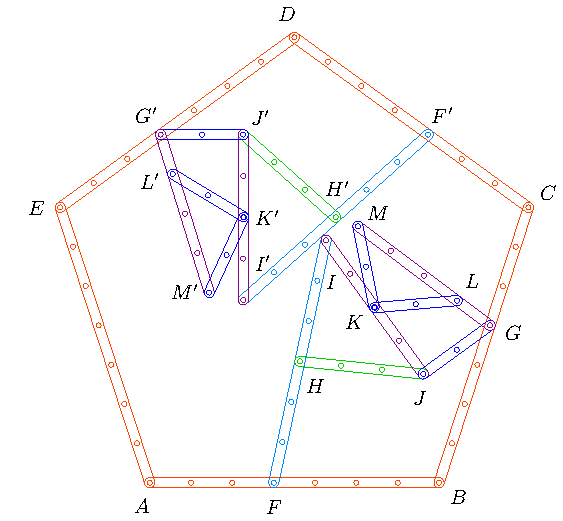
\includegraphics[scale=1]{7/penta7-14a}
\caption{Pentagon of size 7 with 14 internal strips. $\overline{FB} : \overline{BG} = 4:4$ and $\overline{FG} = 2 + 2\sqrt5$.}
\label{fig:penta7-14a}
\end{figure}

Figure \ref{fig:penta7-14a} show pentagon $ABCDE$ of size $7$. We notice an (incomplete) sub-pentagon of size $4$ with two consecutive sides $\overline{FB}$ and $\overline{BG}$. We know the \textbf{widht} of this sub-pentagon is $\dfrac{1+\sqrt5}{2}$ times the sub-side so here:
\begin{align}
\overline{FG} = (4)\frac{1 + \sqrt5}2 = 2 + 2\sqrt5
\end{align}

\subsubsection{Rigid distance $2 + 2\sqrt5$}

Consider the cluster $GLMK$ in figure \ref{fig:penta7-14a}. First we calculate angle $\theta \equiv \angle{LMK}$ with the law of cosines and use this angle to calculate $\overline{KG}$ with the law of cosines:
\begin{align}
\cos\theta &= \frac{(\overline{ML})^2 + (\overline{MK})^2 - (\overline{KL})^2}
 {2(\overline{ML})(\overline{ML})}
 = \frac{3^2 + 2^2 - 2^2}{2(3)(2)} = \frac{3}4 \\
\overline{KG} &= \sqrt{(\overline{GM})^2 + (\overline{MK})^2
 - 2(\overline{GM})(\overline{MK})\cos\theta} \nonumber\\
 &= \sqrt{4^2 + 2^2 - (2)(4)(2)\frac{3}4} = 2\sqrt2
\end{align}

Now since $\overline{KG} = 2\sqrt2$ and $\overline{GJ} = \overline{JK} = 2$ we conclude we have a right angle $\angle{GJK} = \pi / 2.$ And we have a second right angle $\angle{FJI} = \pi/2$ since triangle $\triangle{HIJ}$ is isoscelles and $\overline{IF}$ is the double of $\overline{IH}$. From the two right angles at vertice $J$ we conclude vertices $F,J,G$ are collinear and we verify distance $\overline{FG}$:
\begin{align}
\overline{FG} &= \overline{FJ} + \overline{JG} \nonumber\\
 &= \sqrt{(\overline{IF})^2 - (\overline{IJ})^2} + 2
 = \sqrt{6^2 - 4^2} + 2 = 2 + 2\sqrt5 \quad \blacksquare
\end{align}

% 8

\section{Pentagons of size 8}

% 8-6
\subsection{Size 8 with 6 internal strips $build(8:8)$}

\begin{figure}[H]
\centering
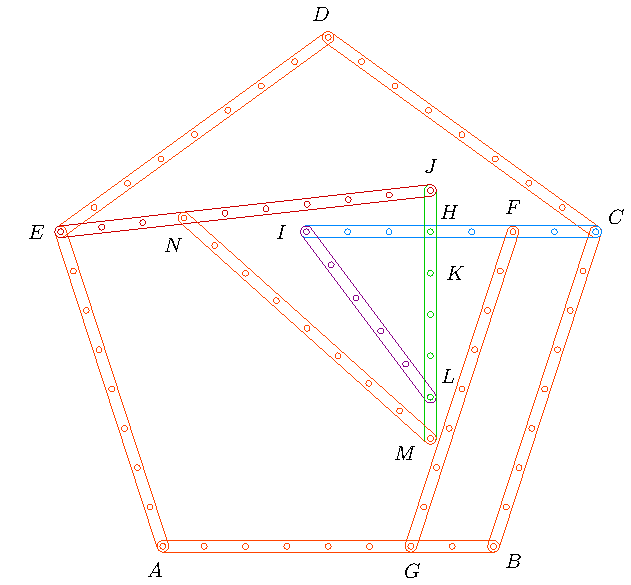
\includegraphics[scale=1]{8/penta8-6a}
\caption{Pentagon of size 8 with 6 internal strips. $\overline{CD} : \overline{DE} = 8:8$. $\overline{FD} = 4 + 4\sqrt5$.}
\label{fig:penta8-6a}
\end{figure}

Figure \ref{fig:penta8-6a} show regular pentagon $ABCDE$ of size 8. We know the pentagon width like $\overline{CE}$ is $\frac{1+\sqrt5}2$ times the side of the pentagon so here we have:
\begin{align}
\overline{CE} &= 8\left(\frac{1 + \sqrt5}2\right) = 4 + 4\sqrt5
\end{align}

We expect vertices $E,H,C$ to be collinear so strip $\overline{FG}$ which is parallel and of the same size that strip $\overline{CB}$ makes rigid the vertices $A$ and $B$.

\subsubsection{Rigid distance $4 + 4\sqrt5$}

From the figure \ref{fig:penta8-6a} consider triangle $\triangle{NJM}$ and calculate with the law of cosines angle $\theta \equiv \angle{NJM}$:
\begin{align}
\cos\theta = \frac{(\overline{JM})^2 + (\overline{JN})^2 
 - (\overline{MN})^2}{2(\overline{JM})(\overline{JN})}
 &= \frac{6^2 + 6^2 - 8^2}{2(6)(6)} = \frac{1}9
\end{align}
Since $\dfrac{\overline{EH}}{\overline{EJ}} = \sin\theta$ we have:
\begin{align}
\overline{EH} &= (\overline{EJ})\sin\theta
 = 9\sqrt{1-\cos^2\theta} 
 = 9\sqrt{1-\left(\frac{1}9\right)^2} = 4\sqrt5
\end{align}

Since $(\overline{EJ})^2 = (\overline{EH})^2 + (\overline{HJ})^2 \mapsto 9^2 = 16(5) + 1$ we found a first right angle $\angle{EHJ} = \pi / 2$. By inspection we have a second right angle $\angle{IHL} = \pi / 2$ formed by the Pythagorean triangle $\triangle{HIL}$ and a third one $\angle{LHC} = \pi / 2$ since is supplementary of $\angle{IHL}$. From the right angles we conclude vertices $E,H,C$ are colinear so we verify the distance $\overline{EH}$:
\begin{align}
\overline{EH} &= \overline{EH} + \overline{HC} = 4 + 4\sqrt{5} \quad \blacksquare
\end{align}

% 8-8
\subsection{Size 8 with 8 internal strips $build(4:8:2:4)$ and $build(4:8:4:6)$}

\begin{figure}[H]
\centering
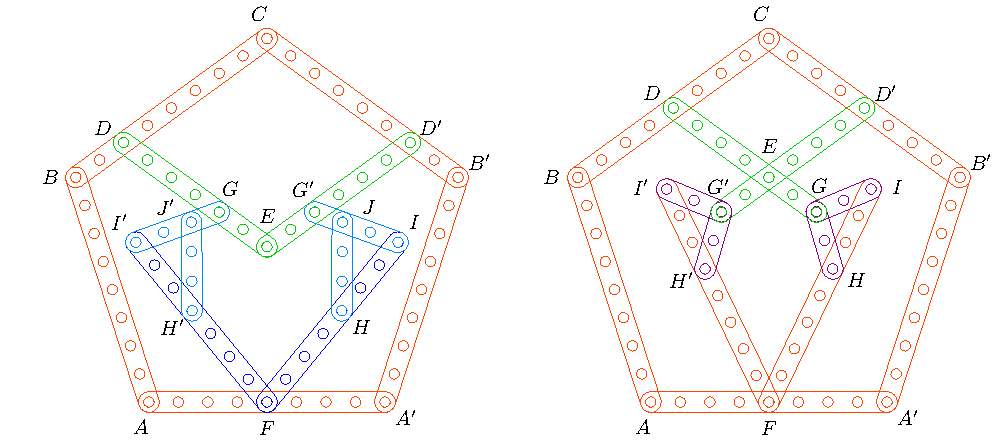
\includegraphics[scale=1]{8/penta8-8a}
\caption{Pentagons of size 8 with 8 internal strips. For pentagon at $(a)$ $\overline{FA}:\overline{AB}:\overline{BD}:\overline{DG} = 4:8:2:4$ and $\overline{FG}=2\sqrt{11}$. For pentagon at $(b)$ $\overline{AF}:\overline{AB}:\overline{BD}:\overline{DG} = 4:8:4:6$ and $\overline{FG}=2\sqrt{11}$.}
\label{fig:penta8-8a}
\end{figure}

Figure \ref{fig:penta8-8a} show two rigid regular pentagons $A,A',B',C,B$ of size $9$. For the pentagon at $(a)$ we assume vertice $F$ is at the origin and calculate the distance $\overline{FG}$ using the abscissas and ordinates following the vertices $FABDG$ for a regular pentagon angles $\alpha = 3\pi/5$, $\beta=\pi/5$:
\begin{align}
FI_x &= -\overline{AF} - \overline{AB}|\cos\alpha| + (\overline{BD} + \overline{DI})\cos\beta\nonumber\\
 &= -4 -(8)\frac{\sqrt5-1}4 + (2+4)\frac{\sqrt5+1}4 = -\frac{2+2\sqrt5}4\\
FI_y &= \overline{AB}\sin\alpha + (\overline{BD}-\overline{DI})\sin\beta\nonumber\\
 &= (8)\frac{\sqrt{10+2\sqrt5}}4 + (2-4)\frac{\sqrt{10-2\sqrt5}}4
 = \frac{8\sqrt{10+2\sqrt5} - 2\sqrt{10-2\sqrt5}}4\\
\overline{FI} &= \sqrt{(FI_x)^2 + (FI_y)^2}\nonumber\\
 &= \frac{\sqrt{(2+2\sqrt5)^2 + (8\sqrt{10+2\sqrt5} - 2\sqrt{10-2\sqrt5})^2}}4
 = \frac{\sqrt{704}}4 = 2\sqrt{11}
\end{align}

For the pentagon at $(b)$ the vertices $G,G'$ switch positions with those of pentagon at $(a)$. In both pentagons we have $\overline{FG} = \overline{FG'} = 2\sqrt{11}$.


\subsubsection{Rigid distances $2\sqrt{11}$}

Our three-strips software found several options for the clusters of pentagons of figure \ref{fig:penta8-8a}. For the pentagon at $(a)$ consider the cluster $FHIJG'$. Within the isoscelles triangle $\triangle{HIJ}$ we calculate the cosine of angle $\theta \equiv \angle{JIH}$ and use it with the law of cosines to verify $\overline{FG'}$:
\begin{align}
\cos\theta &= \frac{\overline{IJ}/2}{\overline{IH}} = \frac{1}3 \nonumber\\
\overline{FG'} &= \sqrt{(\overline{FI})^2 + (\overline{IG'})^2 
 - 2(\overline{FI})(\overline{IG'})\cos\theta} \nonumber\\
 &= \sqrt{7^2 + 3^2 - 2(7)(3)\frac{1}3} = 2\sqrt{11} \quad\blacksquare
\end{align}

For the pentagon at $(b)$ consider the cluster $FHIG$. Within the isoscelles triangle $GIH$ we calculate the cosine of angle $\phi = \angle{HIG}$ and use it with the law of cosines to verify $\overline{FG}$:
\begin{align}
\cos\phi &= \frac{\overline{HI}/2}{\overline{GI}} = \frac{3}4 \nonumber\\
\overline{FH} &= \sqrt{(\overline{FI})^2 + (\overline{GI})^2
 - 2(\overline{FI})(\overline{GI})\cos\phi} \nonumber\\
 &= \sqrt{8^2 + 2^2 - 2(8)(2)\frac{3}4} = 2\sqrt{11} \quad\blacksquare
\end{align}

% 8-10a
\subsection{Size 8 with 10 internal strips $build(4:8)$}

\begin{figure}[H]
\centering
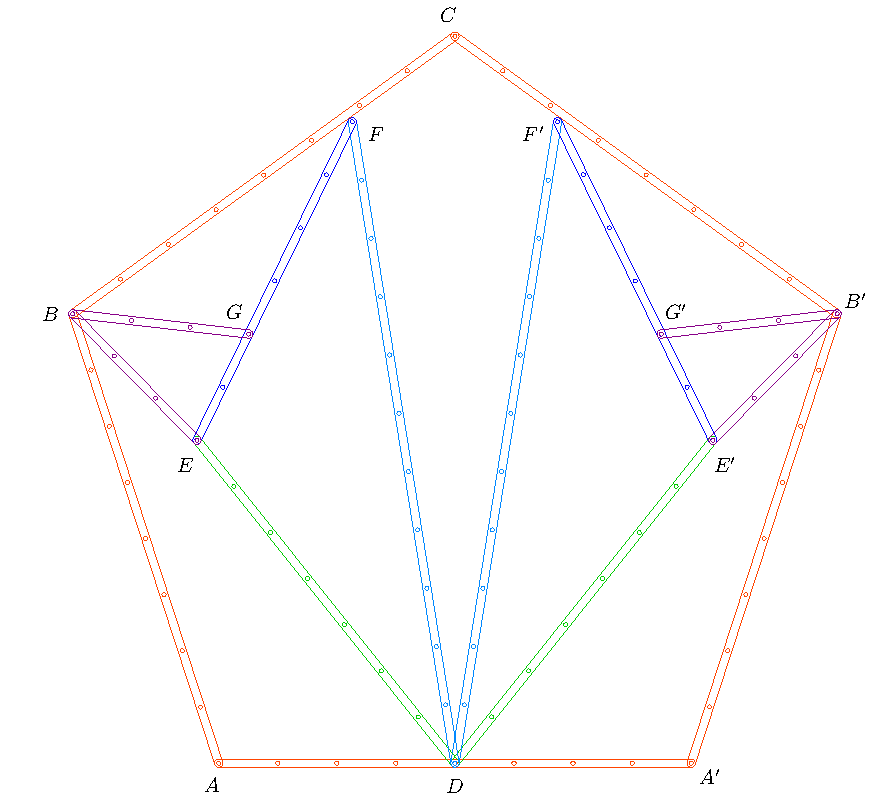
\includegraphics[scale=1]{8/penta8-10a}
\caption{Pentagon of size 8 with 10 internal strips. $\overline{DA}:\overline{AB} = 4:8$ and $\overline{DB} = 4\sqrt{4 + \sqrt5}$}
\label{fig:penta8-10a}
\end{figure}

Figure \ref{fig:penta8-10a} show pentagon $AA'B'CB$ of size $8$. We use the law of cosines to calculate distance $\overline{DB}$. We know $\theta \equiv \angle{DAB} = \dfrac{3\pi}5$ and $\cos\theta = \dfrac{1-\sqrt5}4$ so we have:
\begin{align}
\overline{DB} &= \sqrt{(\overline{AD})^2 + (\overline{AB})^2
 - 2(\overline{AD})(\overline{AB})\cos\theta} \nonumber\\
 &= \sqrt{4^2 + 8^2 - 2(4)(8)\frac{1-\sqrt5}4} = 4\sqrt{4 + \sqrt5}
\end{align}

\subsubsection{Rigid distance $4\sqrt{4 + \sqrt5}$}

Our software found few solutions and the cluster $DEBGF$ shown in the figure \ref{fig:penta8-10a} fit (hardly) inside the pentagon. We calculate two angles around vertice $E$. Angle $\alpha \equiv \angle{DEF}$ whitin the scalene triangle $\triangle{DEF}$ with the law of cosines and angle $\beta \equiv \angle{BEG}$ whitin the isoscelles triangle $\triangle{BEG}$:
\begin{align}
\cos\alpha &= \frac{(\overline{DE})^2 + (\overline{EF})^2 - (\overline{DF})^2}
 {2(\overline{DE})(\overline{EF})} 
 = \frac{7^2 + 6^2 - 11^2}{2(7)(6)} = -\frac{3}7 \\
\sin\alpha &= \sqrt{1 - \cos^2\alpha}
 = \sqrt{1 - \left(-\frac{3}{7}\right)^2} = \frac{2\sqrt{10}}7 \\
\cos\beta &= \frac{\frac{\overline{EG}}2}{\overline{EB}}
 = \frac{\frac{2}{2}}{3} = \frac{1}3\\
\sin\beta &= \sqrt{1 - \sin^2{\beta}}
 = \sqrt{1 - \left(\frac{1}3\right)^2} = \frac{2\sqrt2}3
\end{align}

Finally we calculate the angle $\angle{DEB} = \alpha + \beta$ using the cosines sum identity and use it
to verify the distance $\overline{DB}$:
\begin{align}
\cos(\alpha + \beta) &= \cos\alpha\cos\beta - \sin\alpha\sin\beta \nonumber\\
 &= \left(-\frac{3}7\right)\left(\frac{1}3\right)
  - \left(\frac{2\sqrt{10}}7\right)\left(\frac{2\sqrt2}3\right)
  = -\frac{3 + 8\sqrt{5}}{21} \\
%
\overline{DB} &= \sqrt{(\overline{DE})^2 + (\overline{EB})^2
 - 2(\overline{DE})(\overline{EB})\cos(\alpha + \beta)} \nonumber\\
 &= \sqrt{7^2 + 3^2 - 2(7)(3)\left(-\frac{3 + 8\sqrt{5}}{21}\right)} 
 = 4\sqrt{4 + \sqrt5} \quad\blacksquare
\end{align}

% 8-10b
\subsection{Size 8 with 10 internal strips $build(7:8)$}

\begin{figure}[H]
\centering
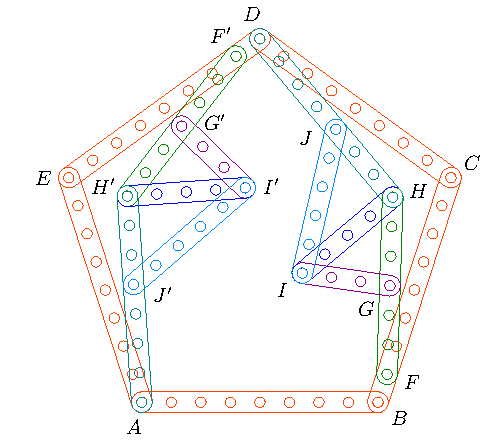
\includegraphics[scale=1.1]{8/penta8-10b}
\caption{Pentagon of size 8 with 10 internal strips. $\overline{FC}:\overline{CD} = 7:8$ and $\overline{FD} = \sqrt{85 + 28\sqrt5}$}
\label{fig:penta8-10b}
\end{figure}

Figure \ref{fig:penta8-10b} show pentagon $ABCDE$ of size $8$. We use the law of cosines to calculate distance $\overline{FD}$ knowing $\theta = \angle{FCD} = \dfrac{3\pi}5$ and $\cos\theta = \dfrac{1-\sqrt5}4$ and calculate angle $\delta \equiv \angle{CFD}$:
\begin{align}
\overline{FD} &= \sqrt{(\overline{FC})^2 + (\overline{CD})^2
 - 2(\overline{FC})(\overline{CD})\cos\theta} \nonumber\\
 &= \sqrt{7^2 + 8^2 - 2(7)(8)\frac{1-\sqrt5}4} = \sqrt{85 + 28\sqrt5} \\
\cos\delta &= \frac{(\overline{FD})^2 + (\overline{FC})^2 - (\overline{CD})^2}
 {2(\overline{FD})(\overline{FC})} \nonumber\\
 &= \frac{85 + 28\sqrt5 + 7^2 - 8^2}{2\sqrt{85 + 28\sqrt5}(7)}
 = \frac{5 + 2\sqrt5}{\sqrt{85 + 28\sqrt5}}
\end{align}

\subsubsection{Rigid distance $\sqrt{85 + 28\sqrt5}$}

Our five-strips software found several solutions, consider the cluster $FGHIJD$ in the figure \ref{fig:penta8-10b}. Assume vertice $I$ is at the origin and vertice $H$ is at coordinate $(4,0)$. Since triangle $\triangle{HIG}$ is isoscelles and $\overline{HF}$ is the double of $\overline{IG}$ then $\overline{IF} = \sqrt{(\overline{HF})^2 - (\overline{IH})^2} = \sqrt{6^2 - 4^2} = 2\sqrt{5}$ and the coordinates of vertice $F$ are $F(x,y) = (0,-\overline{IF}) = (0,-2\sqrt5)$. Since the triangle $\triangle{HIJ}$ is Pythagorean we have a right angle $\angle{IHD} = \pi / 2$ and then the coordinates of vertice $D$ are $D(x,y) = (\overline{IH},\overline{HD}) = (4,7)$. Finally we verify the distance $\overline{FD}$:
\begin{align}
\overline{FD} &= \sqrt{(F_x - D_x)^2 + (F_y - D_y)^2 } \nonumber\\
 &= \sqrt{(0 - 4)^2 + (-2\sqrt5 - 7)^2} = \sqrt{85 + 28\sqrt5} \quad \blacksquare
\end{align}

% 8-10c
\subsection{Size 8 with 10 internal strips $build(8:8)$ and $build(4:8:4)$}

\begin{figure}[H]
\centering
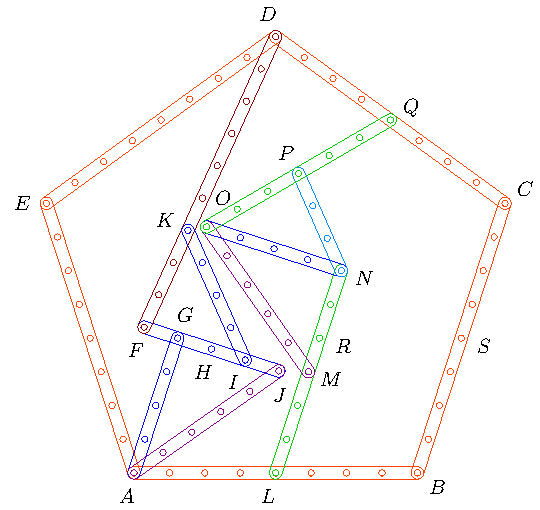
\includegraphics[scale=1]{8/penta8-10c}
\caption{Pentagon of size 8 with 10 internal strips. $\overline{AE}:\overline{ED} = 8:8$ and $\overline{AD} = 4 + 4\sqrt5$. $\overline{LB}:\overline{BC}:\overline{CQ} = 4:8:4$ and $\overline{LQ} = 6 + 2\sqrt5$.}
\label{fig:penta8-10c}
\end{figure}

Figure \ref{fig:penta8-10c} show pentagon $ABCDE$ of size $8$. We have a width $\overline{AD}$ that we know equals the side times $\frac{1+\sqrt5}2$ so we have here:
\begin{align}
\overline{AD} = 8\left(\dfrac{1+\sqrt5}2\right) = 4 + 4\sqrt5
\end{align}
We have a partial sub-pentagon of side $4$ with a semi-perimeter $\overline{RS},\overline{SC},\overline{CQ}$ with width $\overline{RS} = 4\left(\frac{1+\sqrt5}2\right) = 2 + 2\sqrt5$ so we have:
\begin{align}
\overline{LQ} = \overline{LR} + \overline{RQ} = 4 + 2 + 2\sqrt5 = 6 + 2\sqrt5
\end{align}

\subsubsection{Rigid distances $4 + 4\sqrt5$ and $6 + 2\sqrt5$}

From the figure \ref{fig:penta8-10c} we have a (partial) isoscelles triangle $\triangle{FHD}$ where $\alpha = \angle{DFG} = \dfrac{\overline{FG}}{\overline{FD}} = \dfrac{1}9$. The (missing) strip $\overline{HD}$ is substituted by strip $\overline{IK}$ since triangle $\triangle{FIK}$ internal angle $\angle{IFK}$ matches $\alpha$ after using the law of cosines:
\begin{align}
\cos(\angle{IFK}) &= \frac{(\overline{FK})^2 + (\overline{FI})^2 - (\overline{IK})^2}
 {2(\overline{FK})(\overline{FI})} 
 = \frac{3^2 + 3^2 - 4^2}{2(3)(3)}
= \frac{1}9 \quad \blacksquare
\end{align}

Angle $\angle{HGD}= \pi / 2$ since $\triangle{FHD}$ is isoscelles and also $\angle{AGJ} = \pi / 2$ since triangle $\triangle{AGJ}$ is Pythagorean so vertices $A,G,D$ are collinear and then we verify distance $\overline{AD}$:
\begin{align}
\overline{AD} &= \overline{AG} + \overline{GD} \nonumber\\
 &= 4 + \sqrt{(\overline{FD})^2 - (\overline{FG})^2}
 = 4 + \sqrt{9^2 - 1^2} = 4 + 4\sqrt5 \quad \blacksquare
\end{align}

From the figure \ref{fig:penta8-10c} we see triangle $\triangle{NOP}$ is isoscelles and that strip $\overline{OQ}$ is the double of strip $\overline{PN}$ so angle $\angle{ONQ} = \pi / 2$ and we can calculate $\overline{NQ} = \sqrt{(\overline{OQ})^2 - (\overline{ON})^2} = \sqrt{6^2 - 4^2} = 2\sqrt5$. Also angle $\angle{MNO} = \pi / 2$ since triangle $\triangle{MNO}$ is Pythagorean so vertices $M,N,Q$ are collinear and we verify distance $\overline{LQ}$:
\begin{align}
\overline{LQ} &= \overline{LN} + \overline{NQ} \nonumber\\
 &= 6 + 2\sqrt5 \quad \blacksquare
\end{align}


% 9

\section{Pentagons of size 9}

% 9-6
\subsection{Size 9 with 6 internal strips $build(8:9:8)$}

\begin{figure}[H]
 \centering
 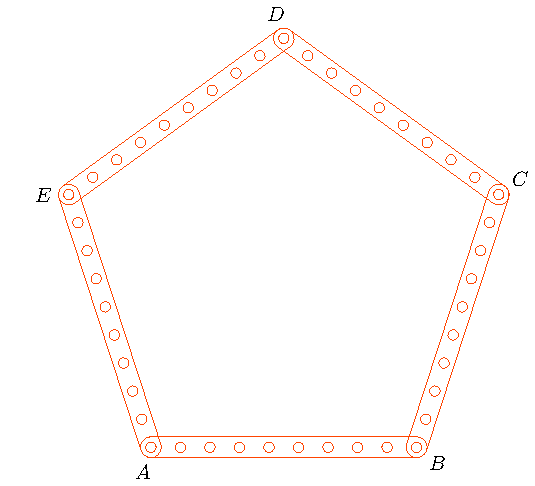
\includegraphics[scale=0.95]{9/penta9a}
 \caption{Pentagon size 9 with six internal strips. $\overline{FB}:\overline{BA}:\overline{AG} = 8:9:8$. $\overline{FG}=5+4\sqrt5$. }
 \label{fig:penta9a}
\end{figure}

Figure \ref{fig:penta9a} show a rigid regular pentagon $A,B,C,D,E$ of size $9$. Inside we have a (partial) sub-pentagon of size $8$ formed with the semi-perimeter of distances $\overline{HS}$, $\overline{SB}$ and $\overline{BF}$. We know the $width$ of the sub-pentagon $\overline{HF}$ equals $\dfrac{1+\sqrt5}2$ times the side of the sub-pentagon so we can calculate the distance $\overline{FG}$:
\begin{align}
\overline{GF} &= \overline{GH} + \overline{HF} \nonumber\\
 &= 8\left(\frac{1+\sqrt5}2\right) + 1 = 5 + 4\sqrt5
\end{align}

We expect here vertices $GJF$ to be collinear so strip $\overline{IN}$ which is parallel and of the same size of segment $\overline{GA}$ makes rigid the vertices $A$ and $B$.

\subsubsection{Rigid distance $5 + 4\sqrt5$}

From the figure we see two right angles. Angle $\angle{GJK} = \pi/2$ because triangle $\triangle{HJK}$  is Pythagorean. Angle $\angle{FJM} = \pi/2$ because triangle $\triangle{FLM}$ is isoscelles. The two right angles share vertice $J$ so vertices $G,J,F$ are collinear. Then we verify the distance $\overline{GF}$:
\begin{align}
\overline{GF} &= \overline{GJ} + \overline{JF} \nonumber\\
 &= 5 + \sqrt{(\overline{LF})^2 - (\overline{LJ})^2} 
 = 5 + \sqrt{9^2-1^2} = 5 + 4\sqrt5 \quad \blacksquare
\end{align}

% 9-8a
\subsection{Size 9 with 8 internal strips $build(3,9,3,5)$}

\begin{figure}[H]
 \centering
 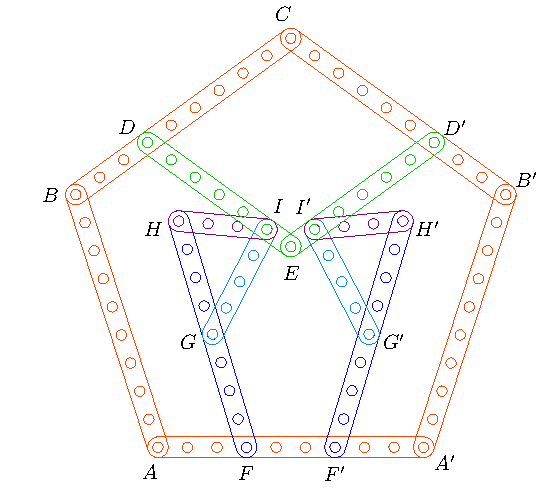
\includegraphics[scale=0.95]{9/penta9-8a}
 \caption{Pentagon size 9 with 8 strips. $\overline{FA}:\overline{AB}:\overline{BD}:\overline{DI} = 3:9:3:5$. $\overline{FI} = \sqrt{55}$.}
 \label{fig:penta9-8a}
\end{figure}

Figure \ref{fig:penta9-8a} show a rigid regular pentagon $A,A',B',C,B$ of size $9$. First we calculate the distance $\overline{FI}$ using the abscissas and ordinates following the vertices sequence $F,A,B,D,I$ with the regular pentagon angles $\alpha \equiv \angle{FAB} = 3\pi/5$, $\beta \equiv \angle{B'BC} = \pi/5$:
\begin{align}
FI_x &= -\overline{AF} - \overline{AB}|\cos\alpha| + (\overline{BD} + \overline{DI})\cos\beta\nonumber\\
 &= -3 - 9\left(\frac{\sqrt5-1}4\right) + (3+5)\frac{\sqrt5+1}4 = \frac{5-\sqrt5}4\\
FI_y &= \overline{AB}\sin\alpha + (\overline{BD}-\overline{DI})\sin\beta\nonumber\\
 &= (9)\frac{\sqrt{10+2\sqrt5}}4 + (3-5)\frac{\sqrt{10-2\sqrt5}}4
 = \frac{9\sqrt{10+2\sqrt5} - 2\sqrt{10-2\sqrt5}}4\\
\overline{FI} &= \sqrt{(FI_x)^2 + (FI_y)^2}\nonumber\\
 &= \frac{\sqrt{(5-\sqrt5)^2 + (9\sqrt{10+2\sqrt5} - 2\sqrt{10-2\sqrt5})^2}}4
 = \frac{\sqrt{880}}4 = \sqrt{55}
\end{align}

\subsubsection{Rigid distance $\sqrt{55}$}

Our three-strips software found the cluster $FGHI$ of figure \ref{fig:penta9-8a}. Triangle $\triangle{GHI}$ is isoscelles and $\overline{FH}$ is the double of $\overline{GH}$ so we have a right angle $\angle{FIH} = \pi/2$ and we confirm the distance $\overline{FI}$:
\begin{align}
\overline{FI} &= \sqrt{(\overline{FH})^2 - (\overline{HI})^2}\nonumber\\
 &= \sqrt{8^2 - 3^2} = \sqrt{55} \quad\blacksquare
\end{align}

% 9-8bc
\subsection{Size 9 with 8 internal strips $build(3,9,1,4)$ and $build(6,9,6,8)$}

\begin{figure}[H]
 \centering
 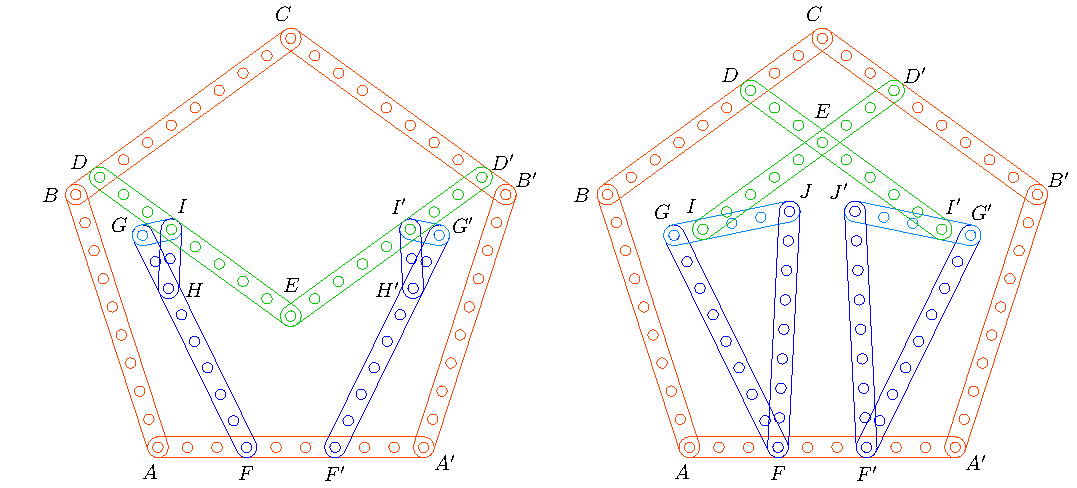
\includegraphics[scale=0.95]{9/penta9-8b}
 \caption{Pentagons size 9 with 8 strips. For the pentagon at $(a)$ we have $\overline{FA}:\overline{AB}:\overline{BD}:\overline{DI} = 3:9:1:4$ and $\overline{FI} = \sqrt{61}$. For pentagon at $(b)$ we have $\overline{F'A}:\overline{AB}:\overline{BD}:\overline{DI'} = 6:9:6:8$ and $\overline{F'I'}=\sqrt{61}$.}
 \label{fig:penta9-8b}
\end{figure}

Figure \ref{fig:penta9-8b} show two pentagons $A,A',B',C,B'$ of size $9$. Both pentagons have the vertices $I,I'$ at the same positions and the same distance $\overline{FI}$. For the pentagon at $(a)$ we calculate using the abscissas and ordinates following the vertices sequence $F,A,B,D,I$ with the regular pentagon angles $\alpha \equiv \angle{FAB} = 3\pi/5$ and $\beta \equiv \angle{B'BC} = \pi/5$:
\begin{align}
FI_x &= -\overline{AF} - \overline{AB}|\cos\alpha| + (\overline{BD} + \overline{DI})\cos\beta\nonumber\\
 &= -3 - 9\left(\frac{\sqrt5-1}4\right) + (1+3)\frac{\sqrt5+1}4 = \frac{1-5\sqrt5}4\\
FI_y &= \overline{AB}\sin\alpha + (\overline{BD}-\overline{DI})\sin\beta\nonumber\\
 &= (9)\frac{\sqrt{10+2\sqrt5}}4 + (1-3)\frac{\sqrt{10-2\sqrt5}}4
 = \frac{9\sqrt{10+2\sqrt5} - 2\sqrt{10-2\sqrt5}}4\\
\overline{FI} &= \sqrt{(FI_x)^2 + (FI_y)^2}\nonumber\\
 &= \frac{\sqrt{(1-\sqrt5)^2 + (9\sqrt{10+2\sqrt5} - 2\sqrt{10-2\sqrt5})^2}}4
 = \frac{\sqrt{976}}4 = \sqrt{61}
\end{align}

\subsubsection{Rigid distance $\sqrt{61}$}

Our three-strips software found several clusters and we use two different for each of the pentagons of figure \ref{fig:penta9-8b}. We calculate the distance $\overline{FI}$ made rigid by clusters $FGHI$ or $FGIJ$ since in both pentagons we have the same sub-triangle $\triangle{FGI}$. With the law of cosines first we calculate $\theta = \angle{FJG}$ and then we confirm $\overline{FI}$:
\begin{align}
\cos\theta &= \frac{\overline{FJ}^2 + \overline{JG}^2 - \overline{GF}^2}
 {2(\overline{FJ})(\overline{JG})}
 = \frac{8^2 + 4^2 - 8^2}{2(8)(4)} = \frac{1}4 \nonumber\\
\overline{FI} &= \sqrt{\overline{IJ}^2 + \overline{FJ}^2 
 - 2(\overline{IJ})(\overline{FJ})\cos\theta} \nonumber\\
 &= \sqrt{3^2 + 8^2 - 2(3)(8)\left(\dfrac{1}4\right)} = \sqrt{61} \quad\blacksquare
\end{align}

% 9-10
\subsection{Size 9 with 10 internal strips $build(4:9)$ and $build(5:9)$}

\begin{figure}[H]
 \centering
 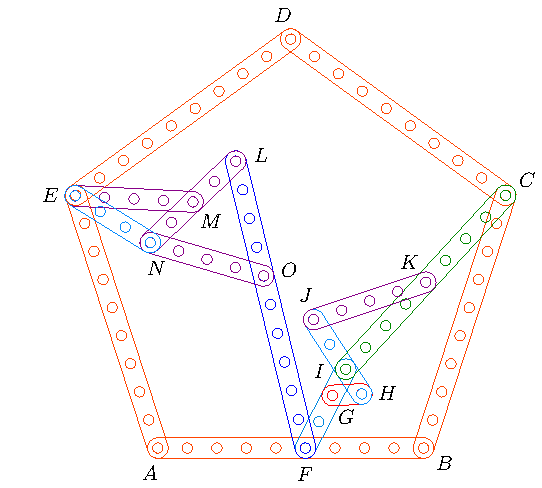
\includegraphics[scale=0.9]{9/penta9b}
 \caption{Pentagons size 9 with two 10 internal strips. For the cluster of the left we have $\overline{FA}:\overline{AE} = 5:9$ and $\overline{FE} = \dfrac{\sqrt{334 + 90\sqrt5}}2$. For the cluster at the right we have $\overline{FB}:\overline{BC} = 4:9$ and $\overline{FC}=\sqrt{79 + 18\sqrt5}$.}
 \label{fig:penta9b}
\end{figure}

Figure \ref{fig:penta9b} show a regular pentagon $A,B,C,D,E$ of size $9$ made it rigid using two different clusters with different distances $\overline{CF}$ and $\overline{EF}$. We calculate the diagonals $\overline{CF}$, $\overline{EF}$ and the angles to side $\overline{AB}$ using the law of cosines and the internal pentagon angle $\theta=\angle{FBC}=\angle{FAE}=\dfrac{3\pi}5$ where $\cos\theta = \dfrac{1-\sqrt5}4$. 

First we calculate distance $\overline{CF}$ and angle $\gamma = \angle{BFC}$:
\begin{align}
\overline{CF} &= \sqrt{
 \overline{BC}^2 + \overline{BF}^2 - 2(\overline{BC})(\overline{BF})\cos\theta } \nonumber\\
 &= \sqrt{9^2 + 4^2 - 2(9)(4)\left(\frac{1-\sqrt5}4\right)} = \sqrt{79 + 18\sqrt5}\\
%
\cos\gamma &= 
 \frac{\overline{CF}^2 + \overline{BF}^2 - \overline{BC}^2}{2(\overline{CF})(\overline{BF})}
 = \frac{79 + 18\sqrt5 + 4^2 - 9^2}{2(\sqrt{79 + 18\sqrt5})(4)}
 = \frac{7 + 9\sqrt5}{4\sqrt{79 + 18\sqrt5}}
\end{align}

Then we calculate $\overline{EF}$ and angle $\epsilon \equiv \angle{AFE}$:
\begin{align}
\overline{EF} &= \sqrt{
 \overline{AE}^2 + \overline{AF}^2 - 2(\overline{AE})(\overline{AF})\cos\theta} \nonumber\\
 &= \sqrt{9^2 + 5^2 - 2(9)(5)\left(\frac{1-\sqrt5}4\right)} = \frac{\sqrt{334 + 90\sqrt5}}2\\
%
\cos\epsilon &=
 \frac{\overline{EF}^2 + \overline{AF}^2 - \overline{EA}^2}{2(\overline{EF})(\overline{AF})}
 = \frac{\dfrac{334 + 90\sqrt5}4 + 5^2 - 9^2 }{2\left(\dfrac{\sqrt{334 + 90\sqrt5}}2\right)(5)}
 = \frac{11 + 9\sqrt5}{2\sqrt{334 + 90\sqrt5}}
\end{align}

\subsubsection{Rigid distance $\sqrt{79 + 18\sqrt5}$}

Our five-strips software found several clusters for distance $\sqrt{79 + 18\sqrt5}$.

\begin{figure}[H]
\centering
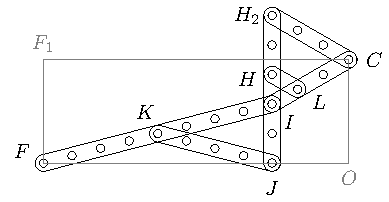
\includegraphics[scale=1]{9/cluster9b1}
\caption{Construction of distance $\overline{FC}=\sqrt{79 + 18\sqrt5}$}
\label{fig:cluster9b1}
\end{figure}

Figure \ref{fig:cluster9b1} show one of several ways to build the distance $\sqrt{79 + 18\sqrt5}$. 
Equilateral triangle $\triangle{FIZ}$ and isosceles $\triangle{IJK}$ share vertice $I$ and the base $\overline{JZ}$ which help to form rectangle $FXCY$ with base $\overline{FX}$ and height $\overline{FY}$ useful to calculate the diagonal $\overline{FC}$:
\begin{align}
\overline{FX} &= \overline{YJ} + \overline{JC}\nonumber\\
 &= \sqrt{\overline{FI}^2 - \left(\frac{\overline{IZ}}2\right)^2}
  + \sqrt{\overline{IC}^2 - \overline{IJ}^2}
  = \sqrt{3^2 - \left(\frac{3}2\right)^2} + \sqrt{8^2 - 2^2} 
  = \frac{3\sqrt3}2 + 2\sqrt{15} \nonumber\\
\overline{FY} &= \overline{JI} + \frac{\overline{IZ}}2
  = 2 + \frac{3}2 = \frac{7}2 \nonumber\\
\overline{FC} &= \sqrt{\overline{FX}^2 + \overline{FY}^2}
 = \sqrt{\left(\frac{3\sqrt3}2 + 2\sqrt{15}\right)^2 + \left(\frac{7}2\right)^2}
 = \sqrt{79 + 18\sqrt5} \quad\blacksquare
\end{align}

We use five strips of this construction with vertices $F,G,H,I,J,K,C$, as a cluster to made rigid the consecutive strips $\overline{AB},\overline{BC}$ of the pentagon of side $9$ of figure \ref{fig:penta9b}.


\subsubsection{Rigid distance $\dfrac{\sqrt{334 + 90\sqrt5}}2$}

Our five-strips software found several clusters for distance$\dfrac{\sqrt{334 + 90\sqrt5}}2$.

\begin{figure}[H]
\centering
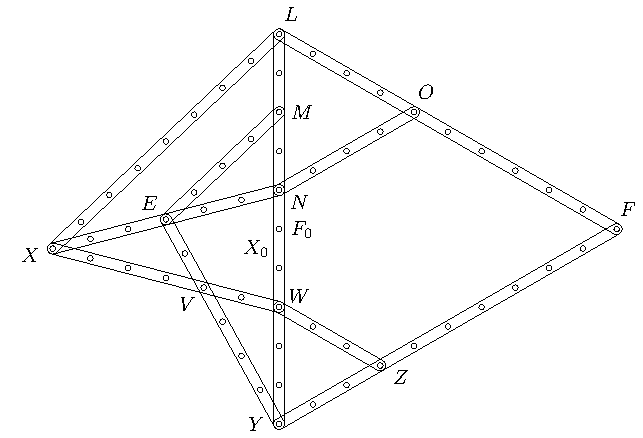
\includegraphics[scale=1]{9/cluster9b2}
\caption{Construction of distance $\overline{EF}=\dfrac{\sqrt{334 + 90\sqrt5}}2$}
\label{fig:cluster9b2}
\end{figure}

Figure \ref{fig:cluster9b2} show equilateral triangle $\triangle{FLY}$ and isoscelles triangle $\triangle{NXW}$ sharing strip $\overline{LY}$ which helps to calculate abscissas and ordinates of vertices $E,F$ to calculate distance $\overline{EF}$. Vertice $Y$ is located at the origin so:
\begin{align}
E_x &= - \left(\frac{\overline{NE}}{\overline{NX}}\right)\overline{XX_0}
 = -\frac{3}6\sqrt{\overline{NX}^2 - \overline{NX_0}^2}
 = -\frac{1}{2}\sqrt{6^2 - \left(\frac{3}2\right)^2} = -\frac{3\sqrt{15}}4 \\
E_y &= \overline{YN} - \left(\frac{\overline{NE}}{\overline{NX}}\right)\overline{NX_0}
 = 6 - \left(\frac{3}6\right)\left(\frac{3}2\right) = \frac{21}4\\
F_x &= \overline{F_0F} = \sqrt{\overline{YF}^2 - \overline{YF_0}^2}
 = \sqrt{10^2 - 5^2} = 5\sqrt3\\
F_y &= \overline{YF_0} = 5\\
\overline{EF} &= \sqrt{(E_x - F_x)^2 + (E_y - F_y)^2} \nonumber\\
 &= \sqrt{\left(-\frac{3\sqrt{15}}{4} -5\sqrt3 \right)^2 + \left(\frac{21}4 - 5\right)^2}
 = \frac{\sqrt{334+90\sqrt5}}2 \quad\blacksquare
\end{align}
We form a cluster from the last construction and insert it inside the pentagon of side $9$. We choose the five strips with vertices $E,N,M,L,O,F$. Is easy to prove strip $\overline{EM}$ is correct in the cluster comparing equal cosines at vertice $Y$ for triangles $\triangle{YVW},\triangle{YEN},\triangle{YEM}$ using the law of cosines for each triangle.


% 10

\section{Pentagon of size 10}

% 10-10
\subsection{Size 10 with 10 internal strips $build(7:10)$}

\begin{figure}[H]
 \centering
 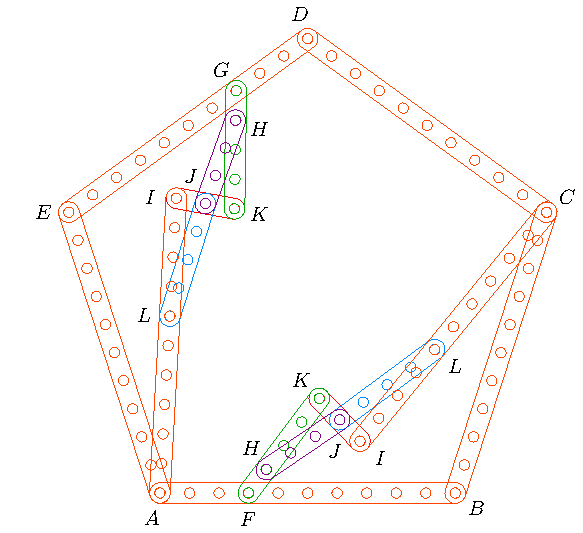
\includegraphics[scale=0.9]{10/penta10a}
 \caption{Pentagon size 10 with 10 interal strips. $\overline{FB}:\overline{BC} = 7:10$ and $\overline{CF} = \sqrt{114 + 35\sqrt5}$.}
 \label{fig:penta10a}
\end{figure}

Figure \ref{fig:penta10a} show a rigid regular pentagon $A,B,C,D,E$ of size 10. We calculate a diagonal joining two consecutive sides relative primes to have something exclusive to the size 10, we choose $\overline{BF}:\overline{BC} = 7:10$. With the law of cosines we calculate $\overline{CF}$.
We calculate the angle $\angle{CFB}$ for the drawing:
\begin{align}
\overline{CF}^2 &= \overline{BC}^2 + \overline{BF}^2
 - 2(\overline{BC})(\overline{BF})\cos\left(\frac{3\pi}5\right) \nonumber\\
 &= 10^2 + 7^2 - 2(10)(7)\left(\frac{1-\sqrt5}4\right) = 114 + 35\sqrt5 \nonumber\\
\overline{CF} &= \sqrt{114 + 35\sqrt5} \\
\cos(\angle{CFB}) &= \frac{\overline{CF}^2 + \overline{BF}^2 - \overline{BC}^2}
 {2(\overline{CF})(\overline{BF})}%\nonumber\\
 = \frac{114+35\sqrt5 + 7^2 - 10^2}{2(\sqrt{114 + 35\sqrt5})(7)}
  = \frac{9+5\sqrt5}{2\sqrt{114+35\sqrt5}}
\end{align}

\subsubsection{Rigid distance $\sqrt{114+35\sqrt5}$}

\begin{figure}[H]
 \centering
 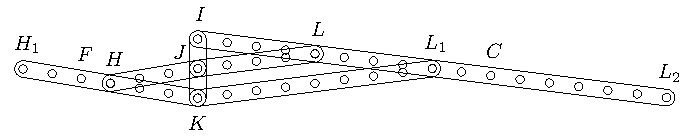
\includegraphics[scale=1.3]{10/cluster10a}
 \caption{Construction of distance $\overline{CF} = \sqrt{114+35\sqrt5}$}
 \label{fig:cluster10a}
\end{figure}

Our software found several solutions for this distance using five strips, and we choose one narrow enough to fit inside the pentagon.
\\\\
Figure \ref{fig:cluster10a} shows how to prove the cluster selected is correct. In the figure we have two isoscelles triangles $\triangle{IKL_1}$ and $\triangle{JKH}$. The sides $IL_1$ and $KH$ are extended to double the original size to the vertices $L_2$ and $H_1$ building two right angles $\angle{IKL_2}$ and $\angle{KJH_1}$. The right triangles permit the calculation of the abscissas and ordinates of vertices $C$ and $F$ to calculate their distance.
\\\\
From the figure we calculate $\overline{KL_2}$ and $\overline{JH_1}$ from their respective right triangles:
\begin{align}
\overline{KL_2} = \sqrt{(\overline{IL_2})^2 - (IK)^2} = \sqrt{16^2 - 2^2} = 6\sqrt7\\
\overline{JH_1} = \sqrt{(\overline{KH_1})^2 - (KJ)^2} = \sqrt{6^2 - 1^2} = \sqrt{35}
\end{align}

Assuming vertice $K$ is at the origin we can calculate the abscissas $C_x,F_x$ and ordinates $C_y,F_y$ of vertices $C$ and $F$ using as factors $c = \dfrac{\overline{IC}}{\overline{IL_2}} = \dfrac{10}{16} = \dfrac{5}8$ and $f = \dfrac{\overline{KF}}{\overline{KH1}}=\dfrac{4}6 = \dfrac{2}3$:
\begin{align}
C_x &= +c(\overline{KL_2}) = \frac{5}{8}(6\sqrt7) = \frac{15}{4}\sqrt7\\
F_x &= -f(\overline{JH_1}) = -\frac{2}{3}\sqrt{35}\\
C_y &= +(\overline{KI}) - c(\overline{KI}) = 2 - \frac{5}{8}(2) = \frac{3}4\\
F_y &= +f(\overline{KJ}) = \frac{2}{3}(1) = \frac{2}3
\end{align}

Finally we calculate the distance $\overline{CF}$:
\begin{align}
\overline{CF} &= \sqrt{(C_x - F_x)^2 + (C_y - F_y)^2}\nonumber\\
 &= \sqrt{\left(\frac{15}{4}\sqrt7 + \frac{2}{3}\sqrt{35}\right)^2
 + \left(\frac{3}4 - \frac{2}3\right)^2} %\nonumber\\
 %&= \sqrt{\dfrac{1575}{16} + 35\sqrt5 + \dfrac{140}9 + \dfrac{1}{144}} 
 = \sqrt{114+35\sqrt5} \quad\blacksquare
\end{align}
A minimal part with five strips of the construction of figure \ref{fig:cluster10a} including only vertices $F,H,I,J,K,L,C$ is used twice to make rigid the pentagon of side 10 as show in figure \ref{fig:penta10a}.

\subsection{Size 10 with 10 internal strips $build(8:10)$}

\begin{figure}[H]
 \centering
 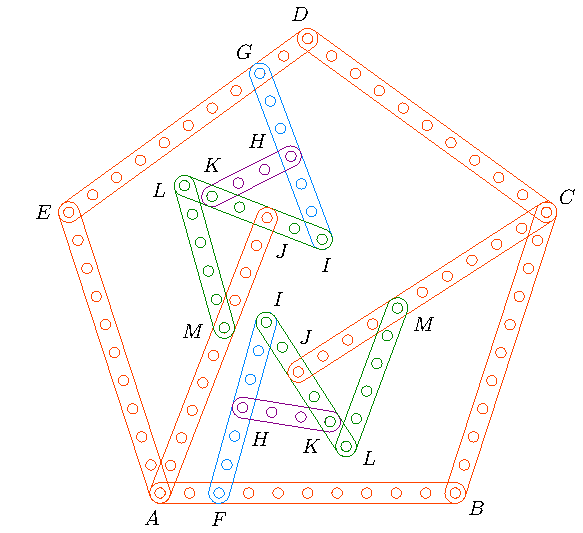
\includegraphics[scale=0.9]{10/penta10b}
 \caption{Pentagon size 10 with 10 internal strips. $\overline{FB}:\overline{BC} = 8:10$ and $\overline{CF} = 2\sqrt{31 + 10\sqrt5}$.}
 \label{fig:penta10b}
\end{figure}

Figure \ref{fig:penta10b} show a rigid regular pentagon $A,B,C,D,E$ of size 10. We include here the relation $\overline{FB}:\overline{BC} = 8:10$ since the relation $4:5$ for pentagon size $5$ gave clusters that can't fit inside such pentagon. With the law of cosines we calculate $\overline{CF}$ and
the angle $\angle{CFB}$ for the drawing:
\begin{align}
\overline{CF}^2 &= \overline{BC}^2 + \overline{BF}^2
 - 2(\overline{BC})(\overline{BF})\cos\left(\frac{3\pi}5\right) \nonumber\\
 &= 10^2 + 8^2 - 2(10)(8)\left(\frac{1-\sqrt5}4\right) = 124 + 40\sqrt5 \nonumber\\
\overline{CF} &= 2\sqrt{31 + 10\sqrt5} \\
\cos(\angle{CFB}) &= \frac{\overline{CF}^2 + \overline{BF}^2 - \overline{BC}^2}
 {2(\overline{CF})(\overline{BF})}%\nonumber\\
 = \frac{124+40\sqrt5 + 8^2 - 10^2}{2(2\sqrt{31 + 10\sqrt5})(8)}
  = \frac{11 + 5\sqrt5}{4\sqrt{31+10\sqrt5}}
\end{align}

\subsubsection{Rigid distance $2\sqrt{31 + 10\sqrt5}$}

One solution from our software is shown in figure as cluster $FHIJKLM$. Assume vertex $J$ is at the origin, vertice $I$ at $(-2,0)$ and vertice $K$ at $(+2,0)$. Since triangle $\triangle{IKH}$ is isoscelles and $\overline{IF}$ is the double of $\overline{IH}$ then angle $\angle{FKI} = \frac{\pi}2$ and we can calculate the abscissa and the ordinate of vertice $F$:
\begin{align}
F_x &= \overline{JK} = 2\\
F_y &= -\sqrt{(\overline{IF})^2 - (\overline{IK})^2} = -\sqrt{6^2 - 4^2} = -2\sqrt5
\end{align}

Since we have the Pythagorean triangle $\triangle{JLM}$ is easy to note that the abscissa and ordinate of vertice $C$ are $C_x = 0$ and $C_y = \overline{JC} = 10$, so finally we have:
\begin{align}
\overline{CF} &= \sqrt{(F_x - C_x)^2 + (F_y - C_y)^2} \nonumber\\
 &= \sqrt{(2 - 0)^2 + (-2\sqrt5 - 10)^2 } = 2\sqrt{31 + 10\sqrt5} \quad\blacksquare
\end{align}

% 11

\section{Pentagon of size 11}

\subsection{Size 11 with 10 internal strips $build(8:11)$}

\begin{figure}[h]
 \centering
 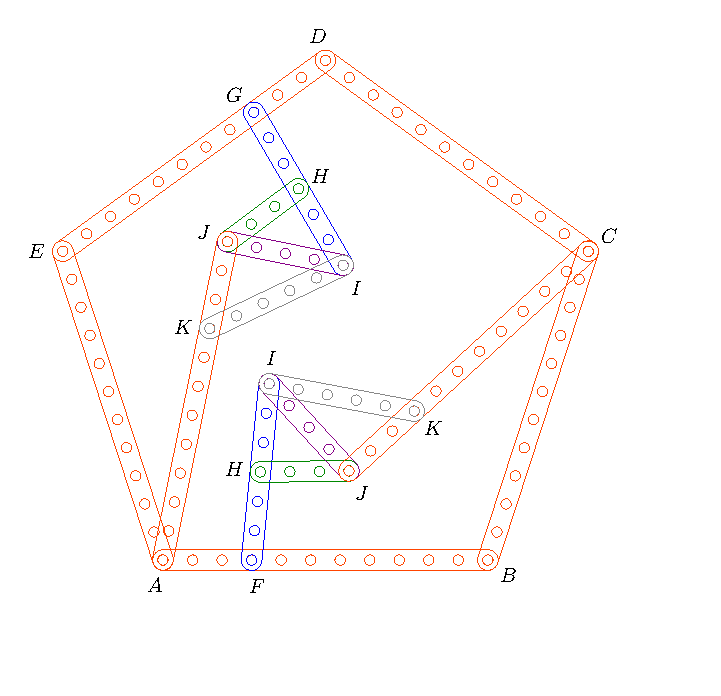
\includegraphics[scale=0.85]{11/penta11a}
 \caption{Pentagon size 11 with 10 internal strips. $\overline{FB}:\overline{BC} = 8:11$ and $\overline{CF} = 11 + 2\sqrt5$.}
 \label{fig:penta11a}
\end{figure}

Figure \ref{fig:penta11a} show a rigid regular pentagon $A,B,C,D,E$ of size 11. Our software found this is the smallest pentagon having a consecutive sides diagonal distance of the form $\dfrac{z_2 + z_3\sqrt5}{z_1}$ instead of the nested form $\dfrac{z_2\sqrt{z_3+z_4\sqrt5}}{z_1}$ where $z_i$ are integers. The mentioned diagonal is the distance $\overline{CF}$ in the figure which can be calculated with the law of cosines knowing angle $\angle{CBF} = \dfrac{3\pi}5$ and denesting the result. We calculate the angle $\angle{CFB}$ for the drawing:
\begin{align}
\overline{CF}^2 &= \overline{BC}^2 + \overline{BF}^2 
 - 2(\overline{BC})(\overline{BF})\cos\left(\dfrac{3\pi}5\right) \nonumber\\
 &= 11^2 + 8^2 - 2(11)(8)\left(\frac{1-\sqrt5}4\right) = 141 + 44\sqrt5 \nonumber\\
\overline{CF} &= \sqrt{141 + 44\sqrt5} \nonumber\\
 &= 11 + 2\sqrt5 \\
%
\cos(\angle{CFB}) &= \frac{\overline{CF}^2 + \overline{BF}^2 - \overline{BC}^2}
 {2(\overline{CF})(\overline{BF})}%\nonumber\\
 = \frac{141+44\sqrt5 + 8^2 - 11^2}{2(11+2\sqrt5)(8)}
  = \frac{21+11\sqrt5}{44+8\sqrt5} = \frac{121+79\sqrt5}{404}
\end{align}

\subsubsection{Rigid istance $11+2\sqrt{5}$}

A five strips cluster can create a rigid distance like $11 + 2\sqrt{5}$. In the figure, three strips $\overline{FI} = 2\overline{HJ}, \overline{FI} > \overline{IJ}$ builds a right angle $\angle{FJI} = \frac{\pi}2$, since triangle $\triangle{IJH}$ is isosceles ($\overline{FH} = \overline{HI} = \overline{JH}$). These three strips also build a distance $\overline{FJ} = \sqrt{\overline{FI}^2 - \overline{IJ}^2} = \sqrt{6^2 - 4^2} = 2\sqrt5$. Now we attach strip $\overline{CJ}$ making a second right triangle $\angle{CJI} = \frac{\pi}2$ using strip $\overline{IK}=5$ as pythagorean diagonal ($\overline{JK}=3, \overline{IJ}=4$). We have two right triangles at vertice $J$ so vertices $F,J,C$ are collinear, so we can calculate the distance $\overline{FC} = \overline{CJ} + \overline{JF} = 11 + 2\sqrt5 \quad\blacksquare$. 

We repeat the five-strips cluster between vertices $A,G$ preventing strips overlaps. Since the clusters are rigid we formed two rigid triangles $\triangle{ABC}, \triangle{DEA}$ so the pentagon is rigid.
\\\\
The software found the next pentagon of this type is a lot bigger: $\overline{BC}=246, \overline{BF}=70, \overline{CF}=41+105\sqrt5$.



% 12

\section{Pentagons of size 12}

\subsection{Size 12 with 4 internal strips $build(0:12:3:4)$}

Our sofware found that side $12$ is the smallest pentagon that can be made rigid with a rhoumbus and two strips as diagonals so need only 4 strips as diagonals.

\begin{figure}[h]
 \centering
 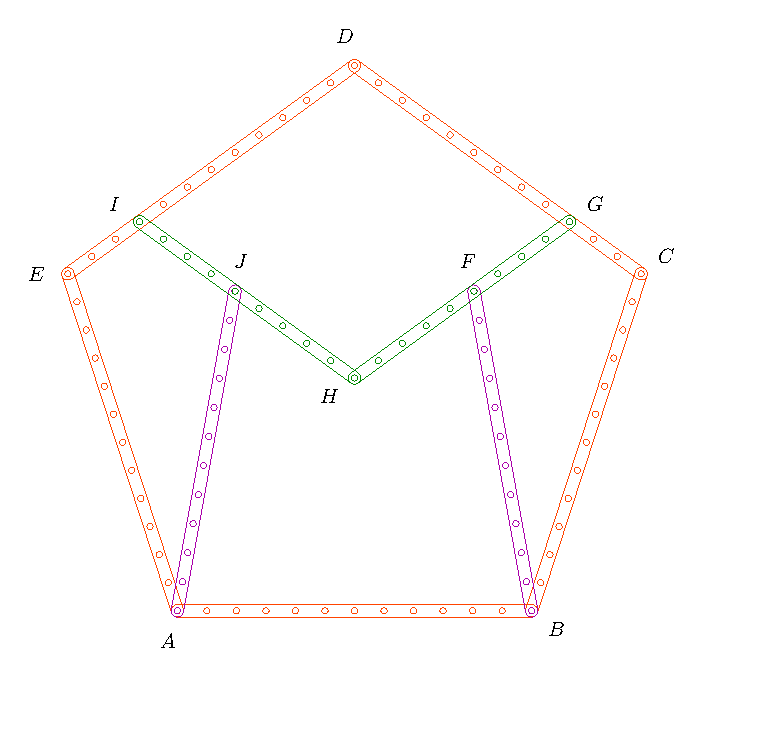
\includegraphics[scale=0.8]{12/penta12a}
 \caption{Pentagon size 12 with 4 internal strips. $\overline{AA}:\overline{AE}:\overline{EI}:\overline{IJ} = 0:12:3:4$ and $\overline{AJ}=11$.}
 \label{fig:penta12a}
\end{figure}

Figure \ref{fig:penta12a} show a regular pentagon $A,B,C,D,E$ of side 12 with a rhombus $D,I,H,G$ of side $9$. We prove strips $AJ,BF$ are correct. First we calculate the abscissas going through vertices $A,E,I,J$ substracting when we move to the left and adding when we move to the right:
\begin{align}
AJ_x &= AE_x + EI_x + IJ_x\nonumber\\
 &= -\overline{AE}\cos\left(\frac{2\pi}5\right)
 + \overline{EI}\cos\left(\frac{\pi}5\right) 
 + \overline{IJ}\cos\left(\frac{\pi}5\right)\nonumber\\
 &= -12\left(\frac{\sqrt5 - 1}4\right)
  +3\left(\frac{1+\sqrt5}4\right)
  +4\left(\frac{1+\sqrt5}4\right) 
  = \frac{19-5\sqrt5}4
\end{align}

Then we calculate the ordinates going to the same order of vertices adding when we go up and substracting when we go down:
\begin{align}
AJ_y &= -AE_y + EI_y + IJ_y\nonumber\\
 &= \overline{AE}\sin\left(\frac{2\pi}5\right)
 + \overline{EI}\sin\left(\frac{\pi}5\right) 
 - \overline{IJ}\sin\left(\frac{\pi}5\right)\nonumber\\
 &= 12\left(\frac{\sqrt{10+2\sqrt5}}4\right)
 + 3\left(\frac{\sqrt{10-2\sqrt5}}4\right)
 - 4\left(\frac{\sqrt{10-2\sqrt5}}4\right)%\nonumber\\
 %&= \frac{12\sqrt{10+2\sqrt5} - \sqrt{10-2\sqrt5}}4 
 = \frac{\sqrt{1450+190\sqrt5}}4
\end{align}
Finally we calculate the distance $\overline{AJ}$ which coincides with strip size $11$:
\begin{align}
\overline{AJ} &= \sqrt{(AJ_x)^2 + (AJ_y)^2}\nonumber\\
 &= \sqrt{\left(\frac{19-5\sqrt5}4\right)^2 + \frac{1450+190\sqrt5}{16}}%\nonumber\\
 %&= \sqrt{\frac{486-190\sqrt5}{16} + \frac{1450+190\sqrt5}{16}} 
 = \sqrt{121} = 11 \quad\blacksquare
\end{align}

\subsection{Size 12 with 4 internal strips $build(4:12:0:3)$}

\begin{figure}[H]
 \centering
 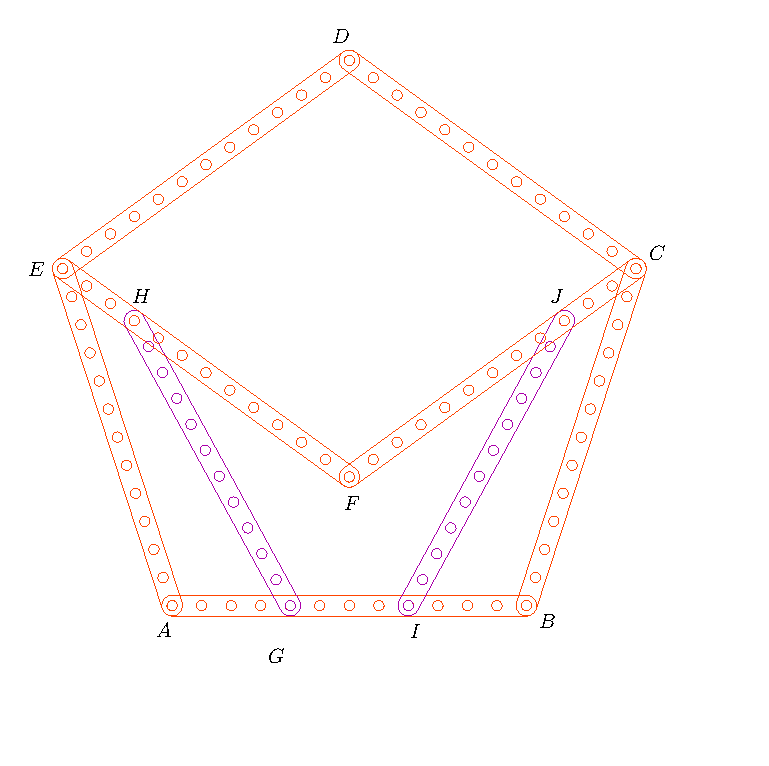
\includegraphics[scale=0.8]{12/penta12b}
 \caption{Pentagon size 12 with 4 internal strips. $\overline{GA}:\overline{AE}:\overline{EE}:\overline{EH} = 4:12:0:3$ and $\overline{GH}=11$.}
 \label{fig:penta12b}
\end{figure}

Figure \ref{fig:penta12b} show a regular pentagon $A,B,C,D,E$ of size 12 with a rhombus $D,I,H,G$ of size $12$. We prove strips $GH,IJ$ are correct. First we calculate the abscissas going through vertices $G,A,E,H$ substracting when we move to the left and adding when we move to the right:
\begin{align}
GH_x &= -GA_x - AE_x + EH_x\nonumber\\
 &= -\overline{GA} - \overline{AE}\cos\left(\frac{2\pi}5\right)
 +\overline{EH}\cos\left(\frac{\pi}5\right)\nonumber\\
 &= -4 - 12\left(\frac{\sqrt5 - 1}4\right) + 3\left(\frac{1+\sqrt5}4\right)
 = \frac{-1-9\sqrt5}4
\end{align}

Then we calculate the ordinates going to the same order of vertices adding when we go up and substracting when we go down:
\begin{align}
GH_y &= AG_y + AE_y - EH_y\nonumber\\
 &= 0 + \overline{AE}\sin\left(\frac{2\pi}5\right)
 - \overline{EH}\sin\left(\frac{\pi}5\right)\nonumber\\
 &= 12\left(\frac{\sqrt{10+2\sqrt5}}4\right)
 - 3\left(\frac{\sqrt{10-2\sqrt5}}4\right)%\nonumber\\
 %&= \frac{12\sqrt{10+2\sqrt5} -3\sqrt{10-2\sqrt5}}4 
 = \frac{\sqrt{1530-18\sqrt5}}4
\end{align}

Finally we calculate the distance $\overline{GH}$ which coincides with strip size $11$:
\begin{align}
\overline{GH} &= \sqrt{(GH_x)^2 + (GH_y)^2}\nonumber\\
 &= \sqrt{\left(\frac{-1-9\sqrt5}{4}\right)^2 + \frac{1530-18\sqrt5}{16}}%\nonumber\\
 %&= \sqrt{\frac{406+18\sqrt5}{16} + \frac{1530-18\sqrt5}{16}} 
 = \sqrt{121} = 11 \quad\blacksquare
\end{align}

\subsection{Size 12 with 6 internal strips $build(12:12)$}

\begin{figure}[h]
 \centering
 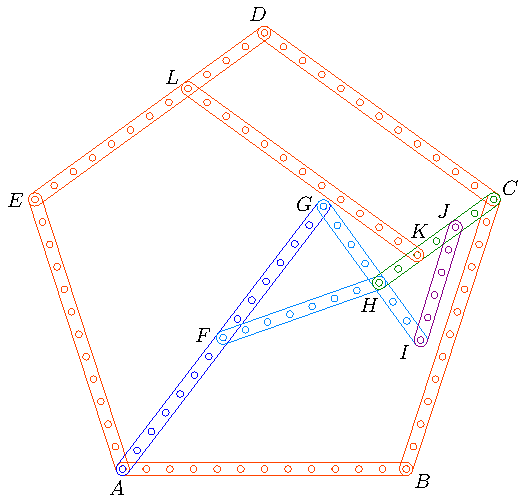
\includegraphics[scale=0.8]{12/penta12-6a}
 \caption{Pentagon size 12 with 6 internal strips. $\overline{AB}:\overline{BC} = 12:12$ and $\overline{AC} = 6 + 6\sqrt5$}.
 \label{fig:penta12-6a}
\end{figure}

Figure \ref{fig:penta12-6a} show a regular pentagon $A,B,C,D,E$ of side 12. We know the regular pentagon diagonal for size 12 is $\overline{AC} = 12\left(\dfrac{1+\sqrt5}2\right) = 6 + 6\sqrt5$. 

\subsubsection{Rigid distance $6 + 6\sqrt5$}

We show the five strips $\overline{GH},\overline{GI},\overline{HF},\overline{HC},\overline{IJ}$ make the diagonal rigid which makes rigid the angle $\angle{ABC}$ of the pentagon. We have an isoscelles triangle $\triangle{FGH}$ and $\overline{AG}$ is two times $\overline{FG}$ so we have a right angle $\angle{AHG} = \frac{\pi}2$ and we can calculate $\overline{AH} = \sqrt{(\overline{AG})^2 - (\overline{GH})^2} = \sqrt{14^2-4^2} = 6\sqrt5$. Now we have another right angle $\angle{IHC} = \frac{\pi}2$ because the Pythagoras triangle $\triangle{HIJ}$. Since $G,H,I$ are collinear then we have another right angle $\angle{GHC}=\frac{\pi}2$. Both right angles $\angle{AHG},\angle{CHG}$ guaranty vertices $A,H,C$ are collinear and we can calculate $\overline{AC} = \overline{AH} + \overline{HC} = 6 + 6\sqrt5$ $\blacksquare$.

Finally we add a sixth strip $\overline{KL}$ parallel to $\overline{CD}$ to make rigid the last three perimeter strips $\overline{CD},\overline{DE},\overline{EA}$ of the pentagon.

\subsection{Size 12 with 8 internal strips $build(6:12:3:6)$}

\begin{figure}[h]
 \centering
 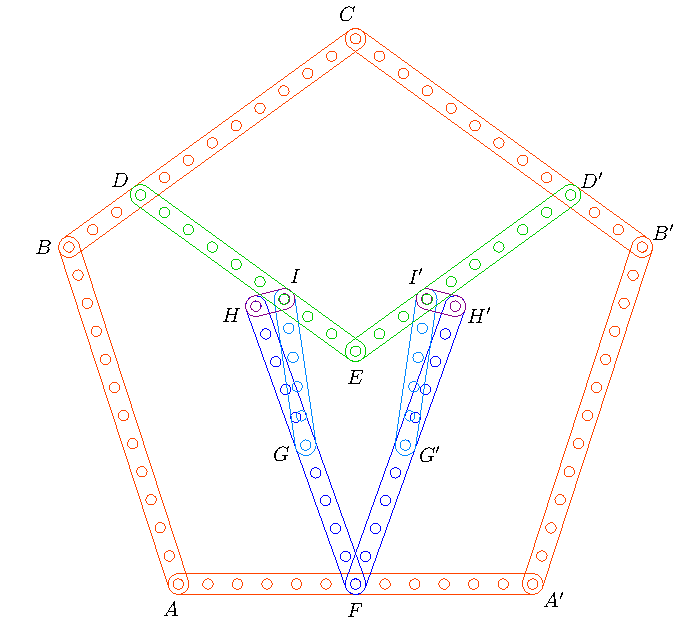
\includegraphics[scale=0.8]{12/penta12-8a}
 \caption{Pentagon size 12 with 8 internal strips. $\overline{FA}:\overline{AB}:\overline{BD}:\overline{DI} = 6:12:3:6$ and $\overline{FI} = 3\sqrt{11}$}.
 \label{fig:penta12-8a}
\end{figure}

Figure \ref{fig:penta12-8a} show a regular pentagon $AA'B'CBA$ of side 12.
First we calculate the distance $\overline{FI}$ using the abscissas and ordinates following the vertices $F,A,B,D,I$ for a regular pentagon angles $\alpha=\dfrac{3\pi}5, \beta=\dfrac{\pi}5$:
\begin{align}
FI_x &= -\overline{AF} - \overline{AB}\cos\alpha + (\overline{BD} + \overline{DI})\cos\beta\nonumber\\
 &= -6 + (12)\frac{1-\sqrt5}4 + (3+6)\frac{\sqrt5+1}4 = -\frac{3+3\sqrt5}4\\
FI_y &= \overline{AB}\sin\alpha + (\overline{BD}-\overline{DI})\sin\beta\nonumber\\
 &= (12)\frac{\sqrt{10+2\sqrt5}}4 + (3-6)\frac{\sqrt{10-2\sqrt5}}4
 = \frac{12\sqrt{10+2\sqrt5} - 3\sqrt{10-2\sqrt5}}4\\
\overline{FI} &= \sqrt{(FI_x)^2 + (FI_y)^2}\nonumber\\
 &= \frac{\sqrt{(-3-3\sqrt5)^2 + (12\sqrt{10+2\sqrt5} - 3\sqrt{10-2\sqrt5})^2}}4
 = \frac{\sqrt{1584}}4 = 3\sqrt{11}
\end{align}

\subsubsection{Rigid distance $3\sqrt{11}$}

Finally we calculate the distance $\overline{FI}$ made rigid by cluster $F,G,H,I$. We have an isoscelles triangle $\triangle{GHI}$ and $\overline{FH}=2\overline{GH}$ so we have a right triangle $\angle{FIH}=\frac{\pi}2$ so: \begin{align}
\overline{FI} &= \sqrt{(\overline{FH})^2 - (\overline{HI})^2}\nonumber\\
 &= \sqrt{10^2 - 1^2} = 3\sqrt{11}
\end{align}

\subsection{Size 12 with 10 internal strips $build(3:12:12)$}

\begin{figure}[H]
 \centering
 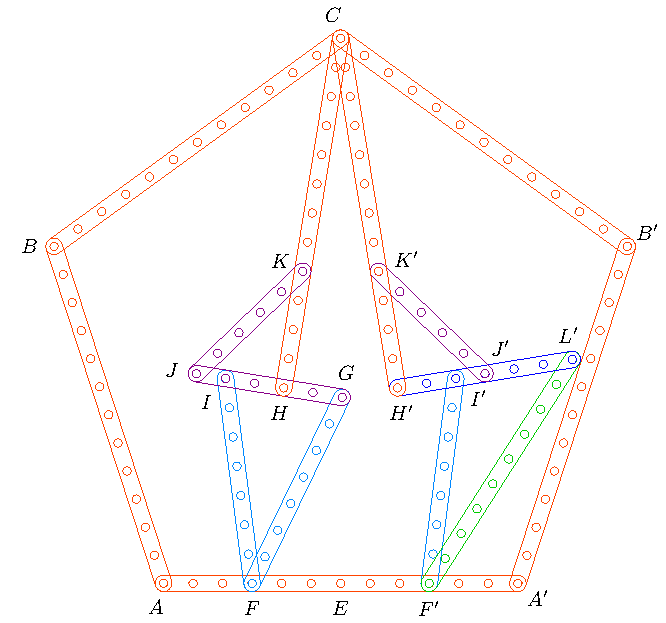
\includegraphics[scale=0.80]{12/penta12-10a}
 \caption{Pentagon size 12 with 10 internal strips.  $\overline{FA}:\overline{AB}:\overline{BC} = 3:12:12$ and $\overline{CF} = 12 + 3\sqrt5$.}
 \label{fig:penta12-10a}
\end{figure}

Figure \ref{fig:penta12-10a} show a regular pentagon $AA'B'CB$ of side 12. We know the regular pentagon height is $\dfrac{\sqrt{5+2\sqrt5}}2$ times the side. So here we have $\overline{CE} = 12\frac{\sqrt{5+2\sqrt5}}2 = 6\sqrt{5+2\sqrt5}$ and we can calculate $\overline{CF}$:
\begin{align}
\overline{CF} &= \sqrt{\overline{CE}^2 + \overline{EF}^2}\nonumber\\
 &= \sqrt{36(5+2\sqrt5) + 3^2} = 3\sqrt{21+8\sqrt5} \nonumber\\
 &= 3(4 + \sqrt5)
\end{align}

\subsubsection{Rigid distance $3(4 + \sqrt5)$}

After testing $\overline{AA'} \le 1800$ our software found that the last denesting is somehow special since other fractions $\dfrac{\overline{AF}}{\overline{AA'}} \neq \dfrac{1}4$ generated $\overline{CF}$s that can't be denested.

We have the Pythagorean triangle $\triangle{HJK}$ and the isoscelles $\triangle{FGI}$ so vertices $FHC$ are collinear. First we calculate $\overline{FH} = \sqrt{\overline{FG}^2 - \overline{GH}^2} = \sqrt{7^2 - 2^2} = 3\sqrt5$ and then $\overline{FC} = \overline{FH} + \overline{HC} = 3\sqrt{5} + 12$ matching last calculation. Finally we prove angle $\angle{F'H'L'} = \frac{\pi}2$ noting $\overline{F'H'} = \sqrt{(\overline{F'L'})^2 - (\overline{H'L'})^2} = \sqrt{9^2 - 6^2} = 3\sqrt5$ matching $\overline{FH}$ $\blacksquare$.

\subsection{Size 12 with 10 internal strips $build(8:12)$}

\begin{figure}[H]
 \centering
 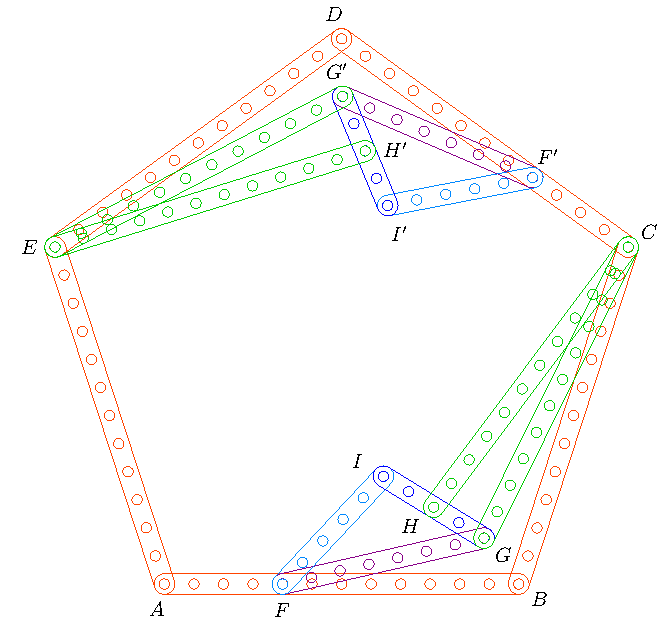
\includegraphics[scale=0.80]{12/penta12-10b}
 \caption{Pentagon size 12 with 10 internal strips.  $\overline{FB}:\overline{BC} = 8:12$ and $\overline{CF} = 4\sqrt{10 + 3\sqrt5}$.}
 \label{fig:penta12-10b}
\end{figure}

Figure \ref{fig:penta12-10b} show a pentagon $ABCDE$ of size $12$. We calculate the distance $\overline{CF}$ with the law of cosines knowing angle $\theta = \angle{CBF} = 3\pi / 5$ and we calculate the angle $\phi = \angle{CFB}$:
\begin{align}
\overline{CF} &= \sqrt{\overline{BC}^2 + \overline{BF}^2 
 - 2(\overline{BC})(\overline{BF})\cos\theta)} \nonumber\\
 &= \sqrt{12^2 + 8^2 - 2(12)(8)\left(\frac{1-\sqrt5}4\right)}
 = 4\sqrt{10 + 3\sqrt5} \\
%
\cos\phi &= \frac{\overline{CF}^2 + \overline{BF}^2 - \overline{BC}^2}
 {2(\overline{CF})(\overline{BF})}%\nonumber\\
 = \frac{16(10 + 3\sqrt5) + 8^2 - 12^2}{2(4\sqrt{10 + 3\sqrt5})(8)}
  = \frac{5 + 3\sqrt5}{4\sqrt{10 + 3\sqrt5}}
\end{align}

\subsubsection{Rigid distance $4\sqrt{10 + 3\sqrt5}$}

Our five-strips software found few options of the form $z_i\sqrt{10+3\sqrt5}$. We validate the cluster $FIHGC$ of figure \ref{fig:penta12-10b}. With the law of cosines we calculate $\alpha = \angle{FGI}$ inside scalene triangle $\triangle{FGI}$ and angle $\beta = \angle{HGC}$ inside isoscelles triangle $\triangle{HGC}$:
\begin{align}
\cos\alpha &= \frac{(\overline{FG})^2 + (\overline{GI})^2 - (\overline{FI})^2}
 {2(\overline{FG})(\overline{GI})}
 = \frac{7^2 + 4^2 - 5^2}{2(7)(4)} = \frac{5}7 \\
\sin\alpha &= \sqrt{1 - \cos^2\alpha} 
 = \sqrt{1 - \left(\frac{5}7\right)^2} = \frac{2\sqrt6}7 \\
\cos\beta &= \frac{\overline{HG}/2}{\overline{GC}} = \frac{1}{11} \\
\sin\beta &= \sqrt{1 - \cos^2\beta}
 = \sqrt{1 - \left(\frac{1}{11}\right)^2} = \frac{2\sqrt{30}}{11}
\end{align}

Finally we calculate angle $\gamma = \alpha + \beta$ using the cosines sum identity and use it to calculate distance $\overline{FC}$ with the law of cosines:
\begin{align}
\cos\gamma &= \cos(\alpha + \beta) = \cos\alpha\cos\beta - \sin\alpha\sin\beta \nonumber\\
 &= \left(\frac{5}7\right)\left(\frac{1}{11}\right) 
  - \left(\frac{2\sqrt6}7\right)\left(\frac{2\sqrt{30}}{11}\right)
  = \frac{5 - 24\sqrt5}{77} \\
%
\overline{FC} &= \sqrt{(\overline{FG})^2 + (\overline{GC})^2 
 - 2(\overline{FG})(\overline{GC})\cos\gamma} \nonumber\\
  &= \sqrt{7^2 + 11^2 - 2(7)(11)\left(\frac{5 - 24\sqrt5}{77}\right)} 
  = 4\sqrt{10 + 3\sqrt5} \quad \blacksquare
\end{align}










\end{document}